\documentclass[10pt,a4paper,twoside]{IEEEtran}
\usepackage[english]{babel}
\usepackage{url}
\usepackage{hyperref}
\usepackage{cite}
\usepackage{listings}
\usepackage{ctable}
\usepackage{amssymb}
\usepackage{graphicx}
\usepackage{amsmath,amssymb}

% \makeatletter
% \let\@ORGmakecaption\@makecaption
% \long\def\@makecaption#1#2{\@ORGmakecaption{#1}{#2}\vskip\belowcaptionskip\relax}
% \makeatother

\author{\IEEEauthorblockN{Anton Bossenbroek \&  Peter van Stralen}\\
\IEEEauthorblockA{Universiteit van Amsterdam\\
email: \tt{\{abossenb, pstralen\}@science.uva.nl}}}
\IEEEpubid{\copyright Copyright 2007 A. Bossenbroek \& P. van Stralen. 
	All text is available under the terms of the GNU Free Documentation
	License}
\title{Solving the TSP through Renormalization and Simulated Annealing}
\begin{document}
\maketitle
\begin{abstract}
We propose a new strategy to solve the euclidean TSP. In the euclidean TSP the goal is to acquire the
shortest tour which visits all the cities specified by a point in the plane. The distance is calculated 
using the euclidean distance. The euclidean TSP is solved using the deterministic renormalization 
method. In renormalization at first a coarse grained route is estimated. This is done by dividing the area
into four cells. The exact shortest route is determined, which connects the cells where at least one city is 
located. This route is refined by recursively dividing each cell and determine the shortest route again. 
If this process is continued until 
each cell contains at most one city, the estimated tour is known. The only problem is how the grid is 
positioned. There is analyzed if thermodynamic simulated annealing can optimize the results found by 
renormalization. In thermodynamic simulated annealing the TSP system is considered as a metal which 
is cooling down. The energy in the system is equal to the length of the tour. In a hot state the rotation can 
be changed significantly. If the metal is becoming colder the allowed rotations on the grid decreases.
This allows to find optimal solutions without getting stuck in a local optima. Our results demonstrate that there
is an improvement of 21 percent over the worst rotation angle. As the number of cities increase, the accuracy
of the estimation decreases only 0.0180 percent per city.  
\end{abstract}
\section{Introduction}
\IEEEPARstart{T}{he} Traveling Sales Person (TSP) problem is a very well known
problem first proposed around 1800 by Sir William Rowan Hamilton and Thomas
Penyngton Kirkman. The problem deals with a traveling salesman which needs to
visit a number of cities. Since time is money, he would like to take the
shortest route possible, but still visit all cities. This is a simple
definition, but TSP is actually a quite large set of combinatorial problems.
Examples of TSP problems are:
\begin{itemize}
\item \textsc{Symmetric TSP problem:}  In this problem there is given a complete graph.
The nodes of these graph are the cities and all cities are connected by
unidirectional edges. The weight of the edge is the distance between the cities.
The task is now to find the shortest tour which visits all cities in the graph,
using each edge at most once (Hamiltonian tour). This tour has to end at the
starting city.
\item \textsc{Euclidean TSP:}  Euclidean TSP problem is a subset of the
Symmetric TSP problem.  Here all the cities are specified by a point in the
plane. The weight of the edges is calculated using the euclidean distance. It
is now again the task to find the shortest Hamiltonian tour.
\item \textsc{Asymmetric TSP problem:} This TSP problem is related to the
Symmetric TSP. In this case we do not have a complete graph and the edges
between the cities are directed.
\item \textsc{Chinese Postmen Problem:} With the Chinese Postmen problem,  the
requirement to find a Hamiltonian tour is somewhat relaxed. It is now allowed
to visit an edge more than once.
\end{itemize}

The TSP problem is interesting from a theoretical aspect as well as from a
practical aspect. Theoretically the TSP problem is NP-hard i.e. it can not be
solved easily. In order to find the optimal solution for the problem all the
possible solutions have to be analyzed. Which can be done in polynomial time.
Better approaches exist to solving a TSP problem, however, the algorithms
which can be used only do an approximation.

Due to the quantity of problems which resemble the TSP problem many attempts
have been made to find the optimal solution. Algorithms which mimic processes
in various disciplines have been used. Examples of such processes are ant
colonies, genetic mutation, neural networks, etc. 

Real space renormalization, a technique from the field of theoretical physics,
has been put forward as a fast approximation technique of the shortest route.
However, this technique relies heavily on the distribution of the cities in
the TSP problem. In this paper we analyze if simulated annealing, a process
which has its analogy from the field of metallurgy, can improve the results
found by renormalization.

This paper is structured as follows. The next section delves deeper in the two
algorithms and motivates the combination. The third section treats the results
found. The last section concludes this work.
\IEEEpubidadjcol % needed for the copyright notice
% vim:ft=tex:spell spelllang=en:autoindent




\section{Renormalization Theory}
\ctable[caption={Studying a problem at multiple scales},
		label={fig:scales},
		figure]{c}{\tnote[]{}}{\FL
			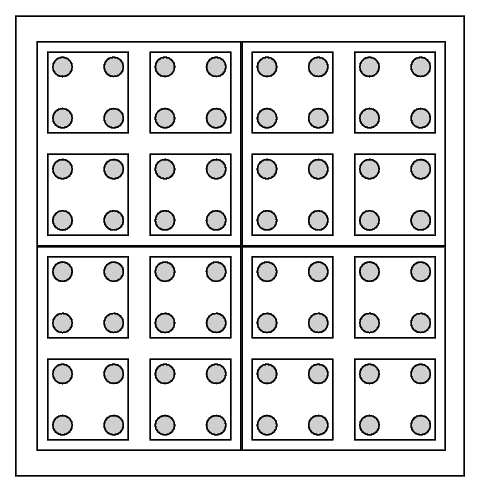
\includegraphics[scale=0.2]{fig/ising.png}
		\LL}
The heart of our method for solving the TSP problem is the renormalization theory. The Renormalization Theory is originating from theoretical physics. In theoretical physics Renormalization is used to study the observe the changes in a physical system. The changes are observed by looking to the problem at different scales. This idea is illustrated in figure \ref{fig:scales}. Here the problem is divided into four parts initially. These parts on their own can again be divided into four parts. This dividing process is repeated until the scale is small enough to study the original problem.

This idea is mapped onto the Traveling Salesman problem. The total square in figure \ref{fig:scales} can be seen as the total area where the cities are located. When estimating the shortest route, we start at a large scale, and we keep zooming in until our estimated optimal tour is known. The procedure is illustrated in figure \ref{fig:renormalization}. The image A is the basic block. This basic block consists of four cells, and can be seen as the four parts in which we divide the problem when we go to a smaller scale. A cell spans a part of the area, and can be enabled or not. The cell is enabled (e.g. needs to be visited) if one or more cities are located in the area spanned by the cell.

The general idea of the algorithm is to solve the Traveling Salesman problem for the larger block. This can be done easily, since a Traveling Salesman problem for at most four cities can be easily solved without much performance penalty, by simply enumerating all possibilities. When this is done, we can look to the TSP at a smaller scale, by dividing the block into four subblocks. Together with some information acquired from the larger block, the Traveling Salesman problem can again be solved for the four subblocks. This process is repeated until there is at most one city in a cell, and the estimated optimal tour is known. In the following subsection we will describes the algorithm in more detail.

\subsection{Preprocessing step}
\ctable[caption={An illustration of how the Renormalization algorithm works},
	label={fig:renormalization},
	figure]{c}{\tnote[]{
	(A) Determine the optimal route in a basic two by two cell. The dashed lines are the edges which can be traversed. The open circles are border points and the closed circles are cell points.\\
	(B) Based on the starting and end border node in a block, lookup the optimal path visiting the cells where at least one city is located.\\
	(C) Divide the block into four subblocks, use the crossings of the route with the borders of a cell (The X) as new starting and end nodes.\\
	(D) These subblocks are treated as a block again, and the process restarts from picture B. This dividing continues until at most one city is in each cell.}}{\FL
	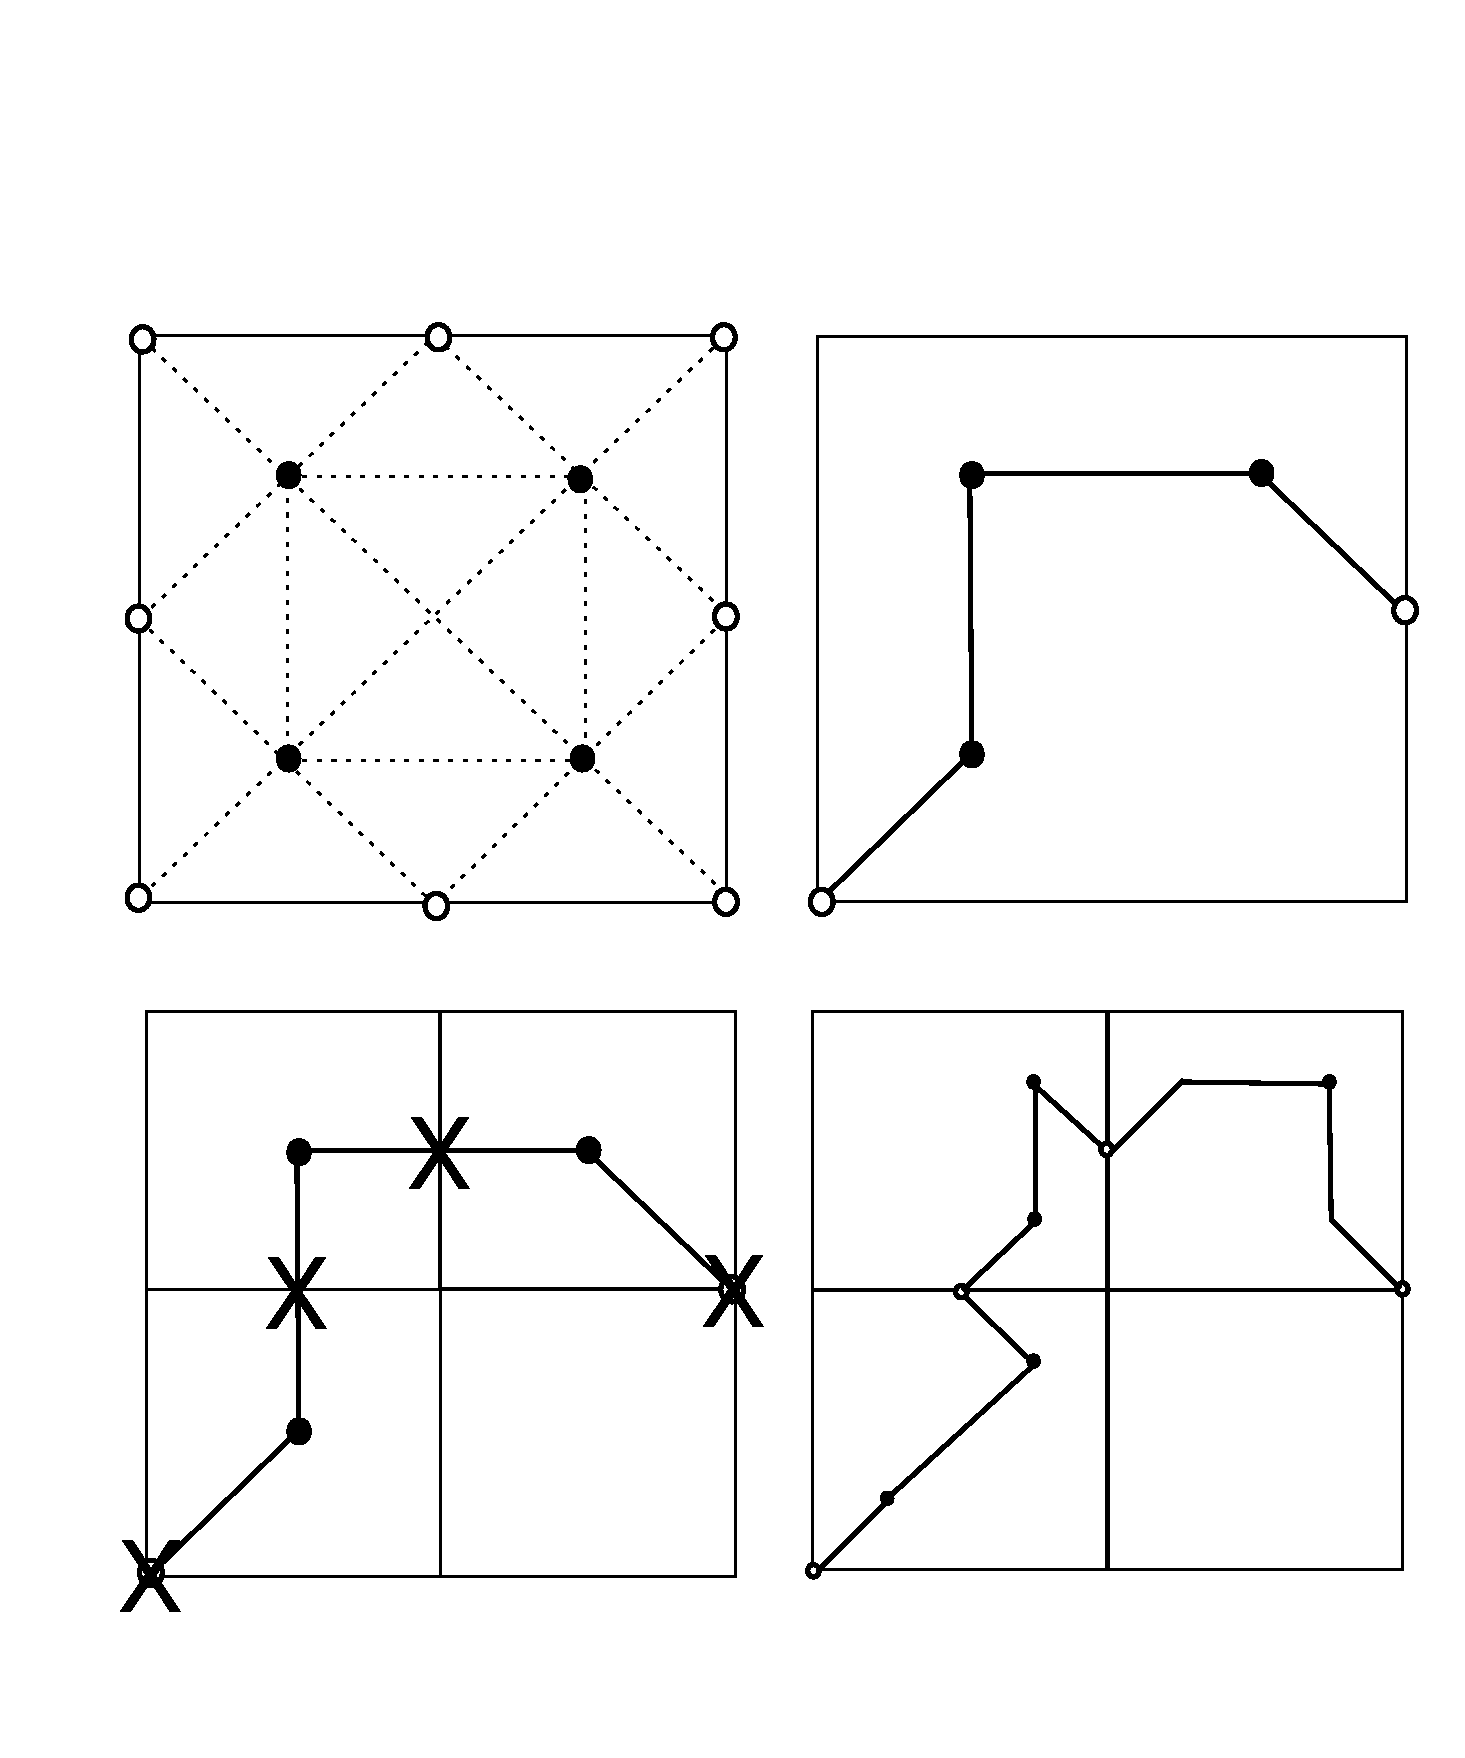
\includegraphics[width=7cm]{fig/renormalization.pdf}
	\LL}

The preprocessing step reduces the amount of calculation needed each time you need to calculate an optimal route in a block. Basically this means that for every possible configuration you calculate the optimal path, and store this in a lookup table. There are two aspects which can be altered, the border point at which the beginning and finish of the route is located and the visited cells within the block.

For retrieving the shortest route through a block, it is considered as a graph. The nodes are the border points and the cell points (Lying in the centrum of a cell). The nodes are connected by multiple edges. There are edges between the border points and the closest cell points. There are also edges from a cell point to the other edges. This set-up can be seen in figure \ref{fig:renormalization}A. For getting the shortest route, a breadth first search is used. Here all possible paths, without cycles, between the starting and end node are calculated. Using these set of paths, the shortest routes visiting subsets of cell points are searched.

\subsection{First iteration}
In the first iteration we start with one block with four cells. In such a block a subset of at least 3 cells needs to be occupied to form a starting tour. The cells where at least one city is located, are connected to form a shortest tour. This tour is an easy connection of the cities, and all the possible routes between them do not need to be investigated.

\subsection{Further iterations}
\ctable[caption={The first four iterations on d198.tsp},
		label={fig:iterations},
		width=7.5cm,
		figure]{cc}{\tnote[]{Some comments}}{\FL
			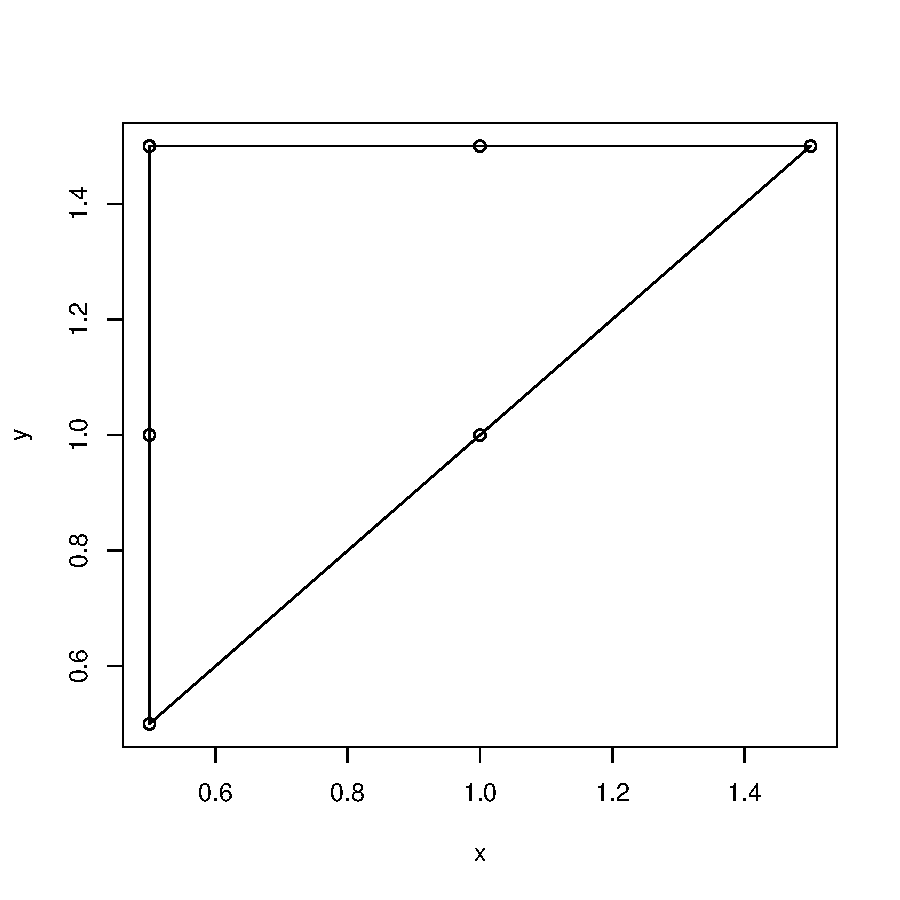
\includegraphics[width=3.5cm]{fig/it2.pdf} &
			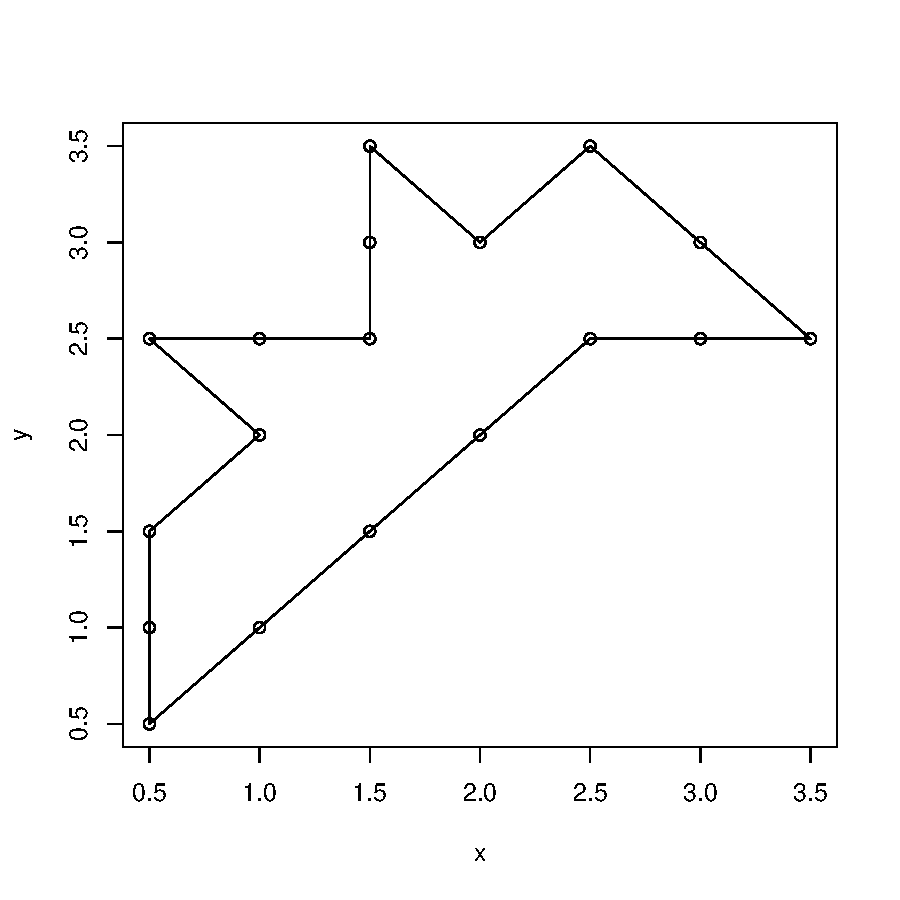
\includegraphics[width=3.5cm]{fig/it4.pdf} \NN
			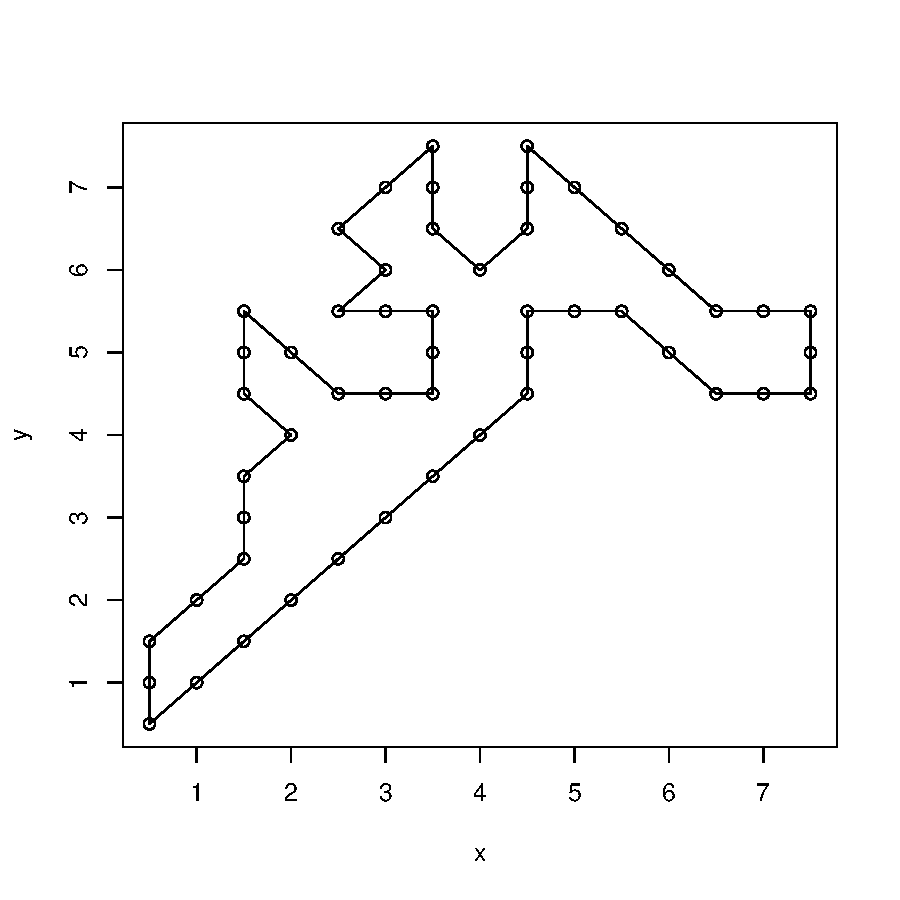
\includegraphics[width=3.5cm]{fig/it8.pdf} &
			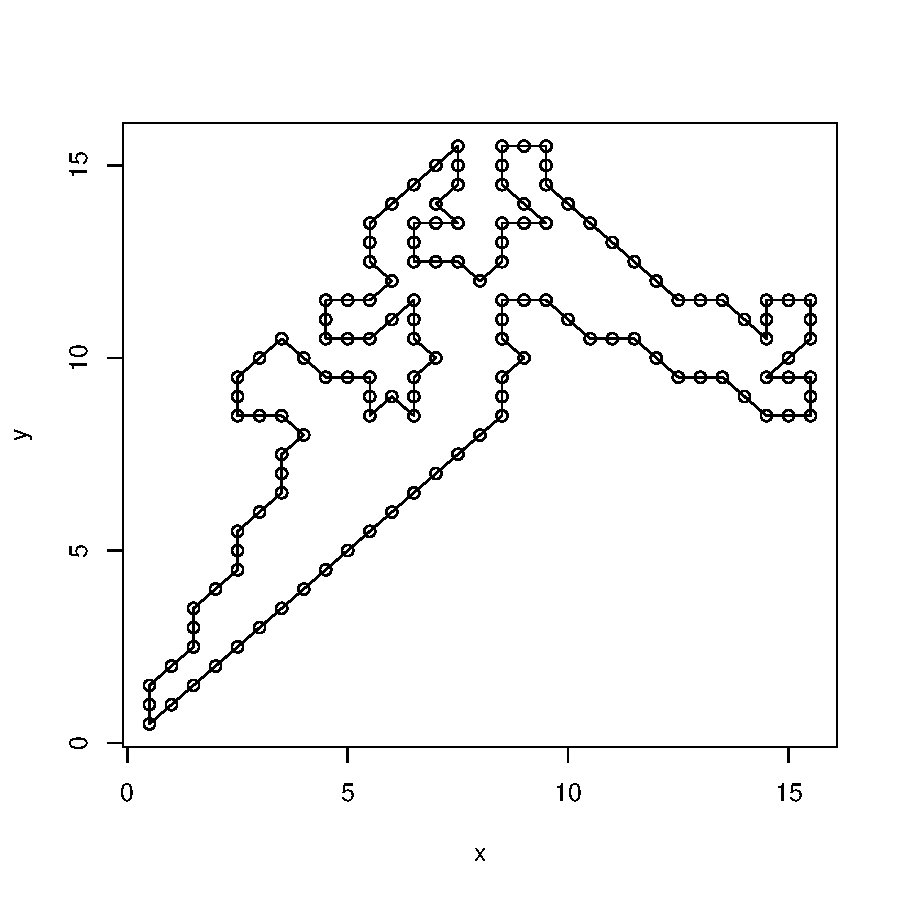
\includegraphics[width=3.5cm]{fig/it16.pdf} 
			\LL}


When the first iteration is finished we can use earlier blocks to calculate an approximation of the shortest tour at a smaller scale. We can divide all the blocks in four subblocks to study the problem at a smaller scale. Instead of iterating over all the subblocks in the image, which can be quite time consuming at a very small scale, only the blocks which are contains at least one city in the previous estimated shortest tour are used in the calculation. This limits the needed memory in the order of the size of the problem.

The information which is retrieved from the previous scale are the crossing points of the previous optimal path through the block. This optimal path can be seen in figure \ref{fig:renormalization}B.  These crossing points are at the places, where the edges of the path, pass the borders of one of the cells. This is illustrated in figure \ref{fig:renormalization}C. These crossing points, precalculated during the preprocessing stage, are used as start and ending point in the subblock. The optimal path between the starting and endpoint is retrieved, and placed in the subblock. The subblock is now a block on its own again, and can be used in the next scale.

\subsection{Retrieving the estimate of the shortest tour}
These process, which looks like zooming in on a microscope, is repeated until we reach unity. Unity is defined as the case where each cell has at most one city in it. Now we can directly retrieve our estimation of the shortest path. In figure \ref{fig:iterations} the first four iterations of the algorithm on $d198.tsp$ is shown. What is clear from this picture is that the route is refined in each iteration, until it exactly maps on the estimation  of the shortest optimal tour.

\subsection{Parallelization}
This algorithm can be extended for parallel execution. We did not perform this extension, but we have a suggestion of how to do this. The foundation for parallelism is in the observation that if we decrease to a smaller scale, we divide all the blocks into four subblocks independently. So if the code needs to be parallelized you take the following steps:

\begin{enumerate}
\item First perform some iterations on a single process. This is done until there are sufficient number of blocks for all the processes
\item Distribute the blocks over the processes, each process should have one connected part of the tour.
\item Each process can now recursively divide these blocks into subblocks, until unity is reached.
\item The cities which are visited in the part of a single process are retrieved and send back to the initiating process. These one can collect the data and output the total tour.
\end{enumerate}

This approach has a high potential of parallelism, since no communication is needed. Their is a pitfall however. If the blocks are shared equally it does not have to mean that the work is equally divided. In a worst case scenario a small group of processes can have a large set of all the cities. This problem can be reduced if there is a process which performs load balancing by shifting blocks, or sending one small set of blocks to a process at the time.
% vim:ft=tex:spell spelllang=en:autoindent

\section{Simulated Annealing}
\subsection{Introduction}
According to \cite{yoshiyuki1995nms} the renormalization algorithm works best
when the cities are uniformly distributed over the pane. It is clear that this
is very unlikely in real TSP optimisation problems. For the United States of
America for example most cities are located on the east coast. The Netherlands
on the other hand have a concentration of cities in the west of the country.
It is clear that the location of the cities cannot be changed without
modifying the problem. We propose to change the distribution of the cities
over the cells in the grid by rotating the grid used by the renormalization
process.

A deterministic algorithm such as a greedy algorithm, can be used to find the
angle of the rotation leading to the best approximation of the shortest route. Yet
deterministic algorithms will succumb to stay in a local optimum and are
therefore inadequate. Probabilistic algorithms can resist to this risk. By
first seeking through the entire sample space multiple optima can be found.
Depending on the algorithm used one or more optima are further analyzed to
find a global optimum.

The thermodynamic simulated annealing (TSA) algorithm
\cite{devicente2003pts}~is the probabilistic algorithm used in this work. This
process is an extension of the simulated annealing (SA) algorithm first
discussed in \cite{kirkpatrick83}. The latter algorithm is analogous to the
process of annealing in metallurgy. First a metal is heated to high
temperature. Once warm it is slowly cooled in a controlled way permitting the
atoms of the metal to fall into an optimal equilibrium and thereby reducing
the energy to a minimum. Because the atoms are in an optimal place the metal
has many ideal properties. 

To use SA first some properties of the system have to be defined to resemble
the physical process. The energy of the system is defined to be the length of
the route found by the renormalization process. The sample space which can be
altered to reduce the energy is the angle of the rotation of the grid.  The
two core elements of the SA process are the cooling schedule which permits to
reduce the energy of the system. The second is the method used to bring the
system in a new disequilibrium. This latter property, to which will be
referred to as the perturbation function, models the dynamic of the atoms
depending of the temperature of the system.

The next subsections treat the perturbation function and the cooling schedule used
to find the optimal angle of the rotation.

\subsection{Perturbation function}
In most SA algorithms the system is brought in a new
disequilibrium by changing the current state by a small fraction. This is hard
to accomplish when rotating the grid used by the renormalization algorithm;
even a very small change of the angle of the rotation can lead to a complete
new route with a much higher or lower energy. Yet if the perturbation function
allows to return in the previously better state this is not a problem. To
implement this behaviour the perturbation function uses a random walk.

\newcommand{\expt}{\ensuremath{\mathbb{E}}}
The random walk used is based on a Brownian motion\cite{brown1829bam}. The
Brownian motion is used, among others, in physics to describe the random
movement of particles suspended in a fluid. The Brownian motion is
a stochastic process $\lbrace W_t\rbrace_{t\geq 0}$ with the properties that
if $\mathcal{F}_t$ denotes the information known until time $t$ then 
$\expt(W_{t + 1}\mid \mathcal{F}_t) = \expt(W_t \mid \mathcal{F}_t)$ i.e. the
expectation of process at the next time step is only dependent on the
information known up to the current time. However the expectation is still
zero. Furthermore, $W_t - W_s \sim N(0, 1)$. Using this process we define the
angle of rotation $\theta_t$ at time $t$ to be:
\begin{equation}\label{eq:rot}
\theta_{t + 1} = \theta_{t} + \alpha 2\pi\frac{T - T_{end}}
	{T_{init} - T_{end}}W_t
\end{equation}
where $T_{init}, T_{end}$ and $T$ are respectively the initial temperature of
the system, the desired end temperature and the current temperature. The
factor $\alpha$ is used to determine how much the rotation should be influenced
by the Brownian motion. The Brownian motion is multiplied by $2\pi$ to ensure
that an entire rotation can be accomplished.

\ctable[caption={The rotation angle over the entire TSA process},
	     figure,
		  label={fig:rotful}]{c}{\tnote[]{The angle is changed using equation
		  \eqref{eq:rot}. Because the temperature remains around the initial
		  level throughout almost the entire time the rotation changes
		  frequently.}}{\FL
		  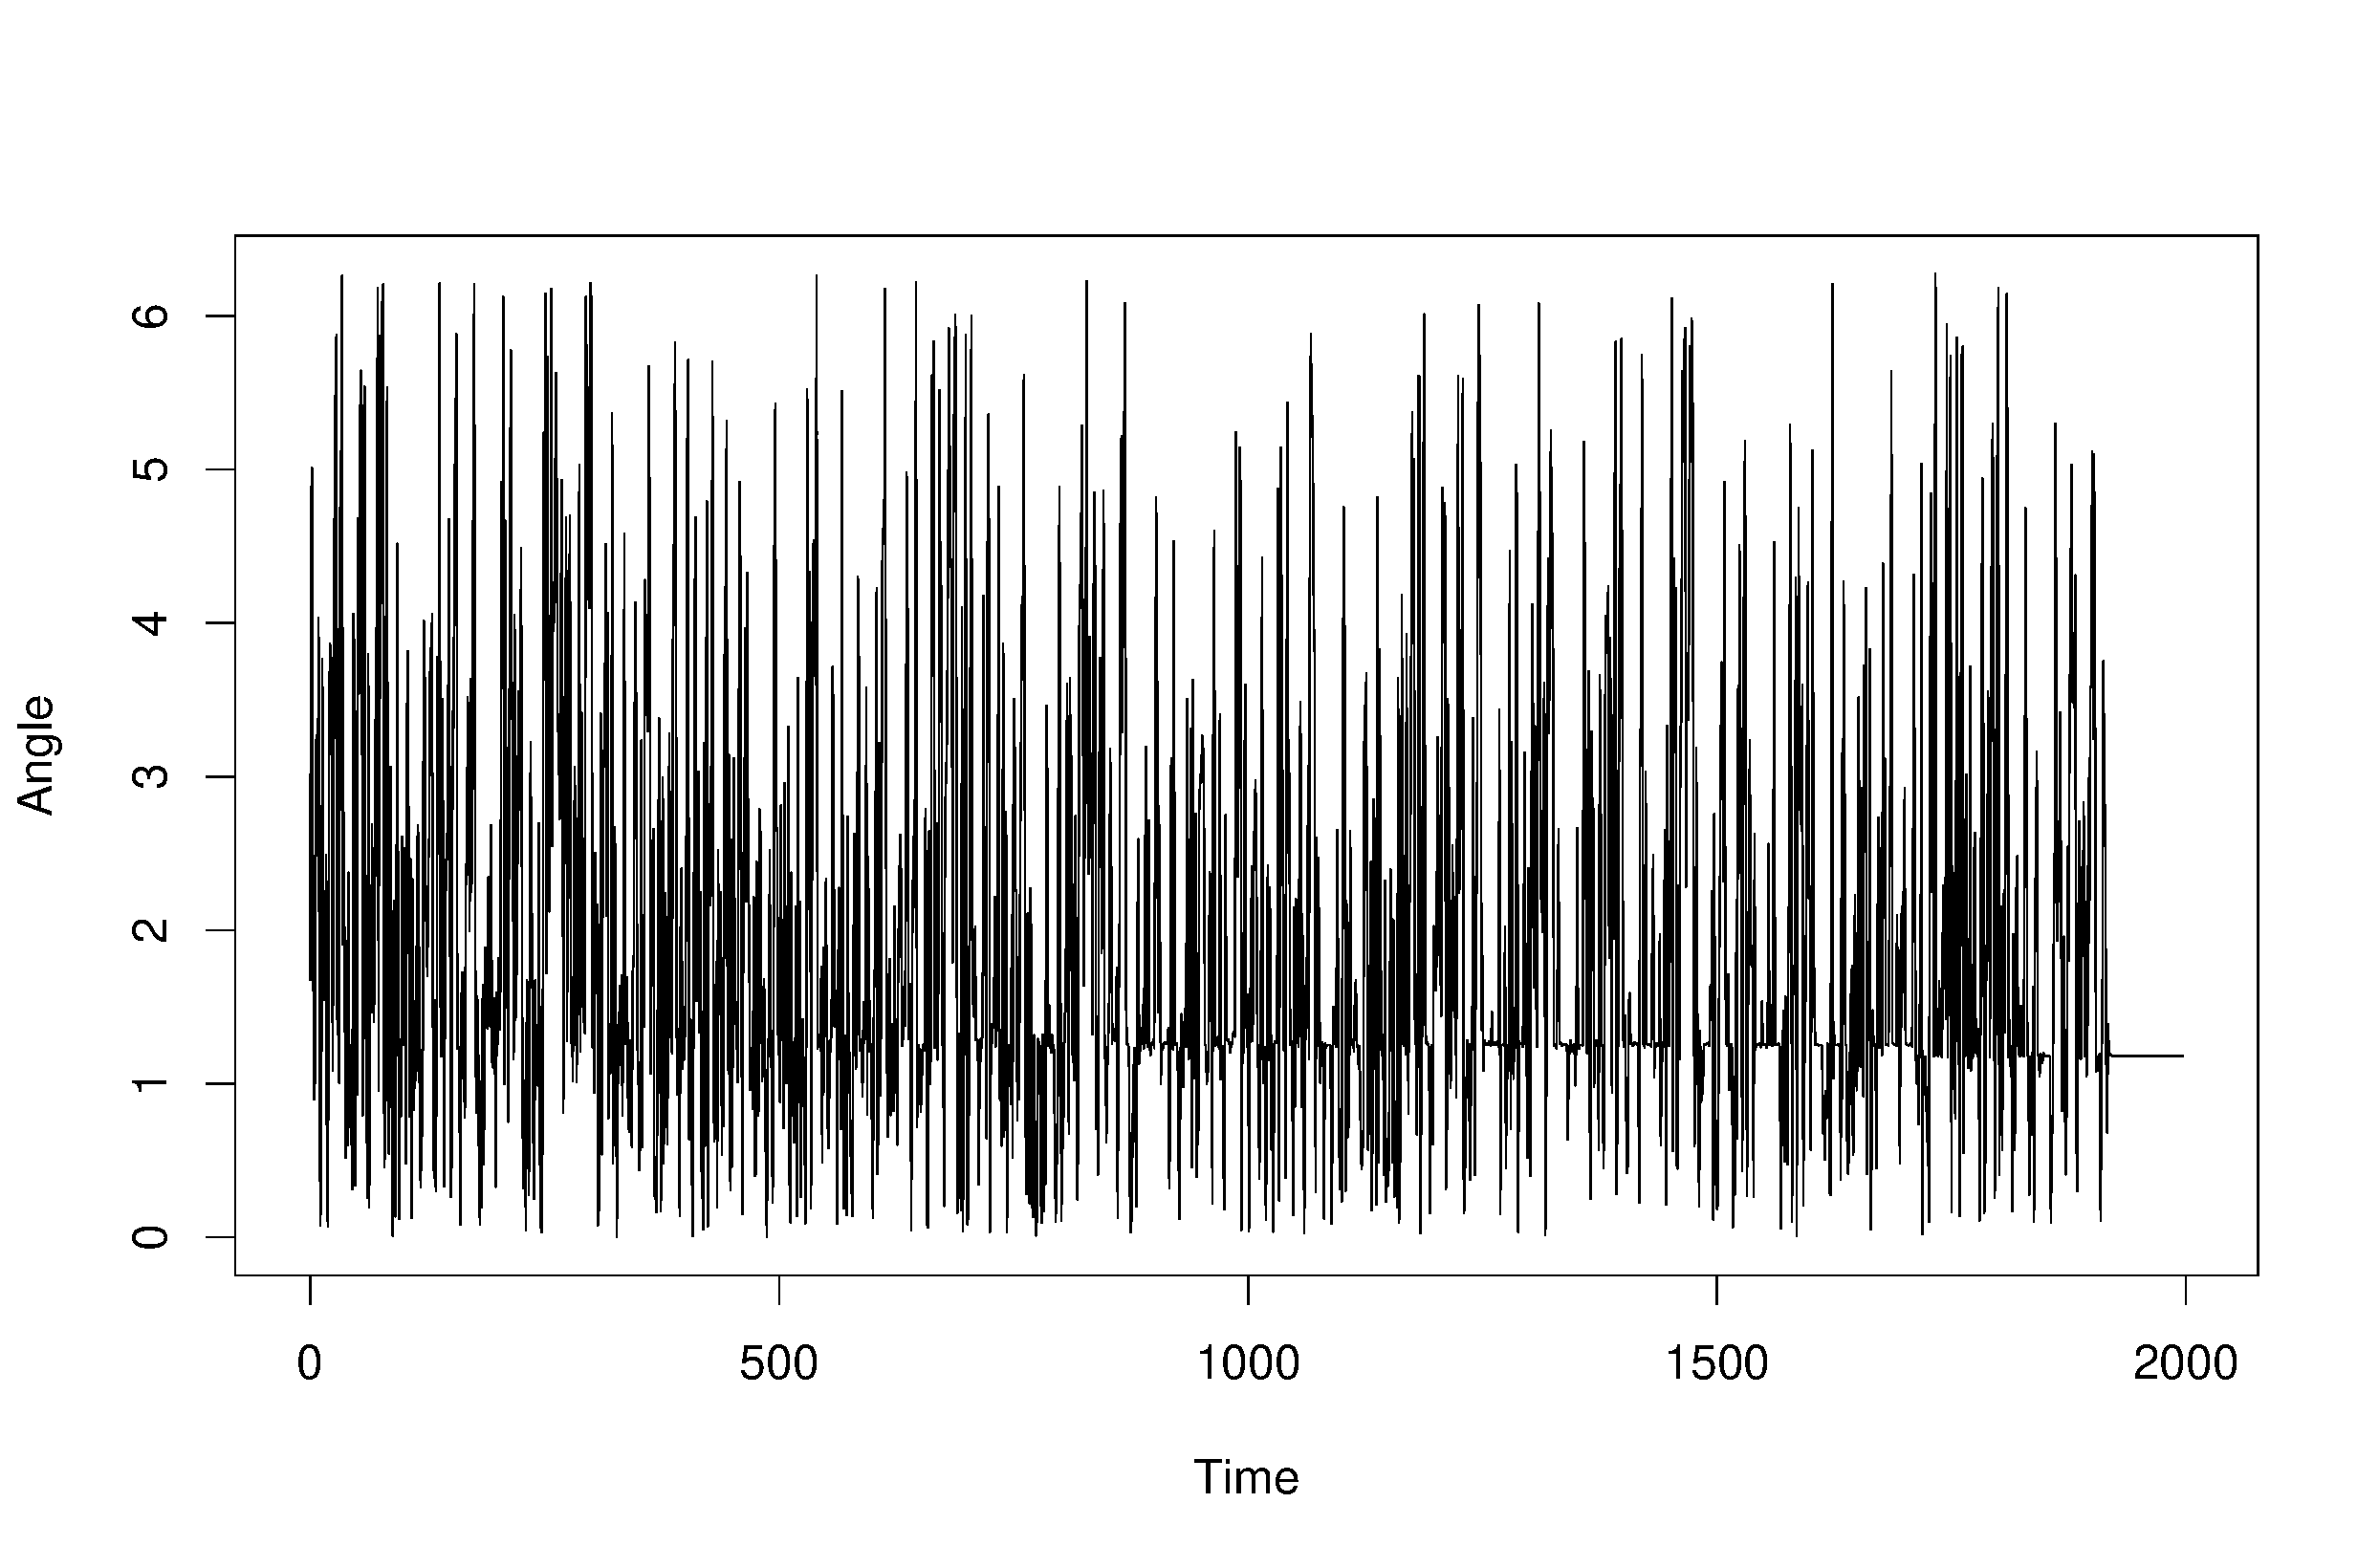
\includegraphics[width=8cm]{fig/rotation_full}\NN
		  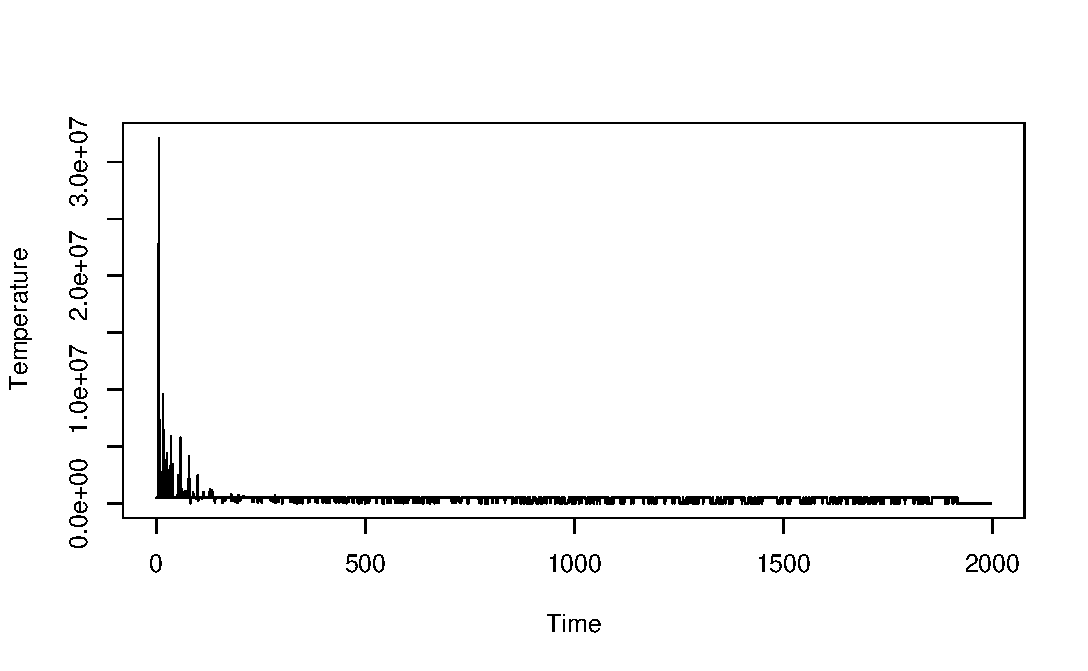
\includegraphics[width=8cm]{fig/temp_rot_full}\LL
		  }

\ctable[caption={The rotation angle over the time period of 400 to 600},
	     figure,
		  label={fig:rot46}]{c}{\tnote[]{The figure shows that while the
		  temperature is high the change of the rotation angle  }}{\FL
		  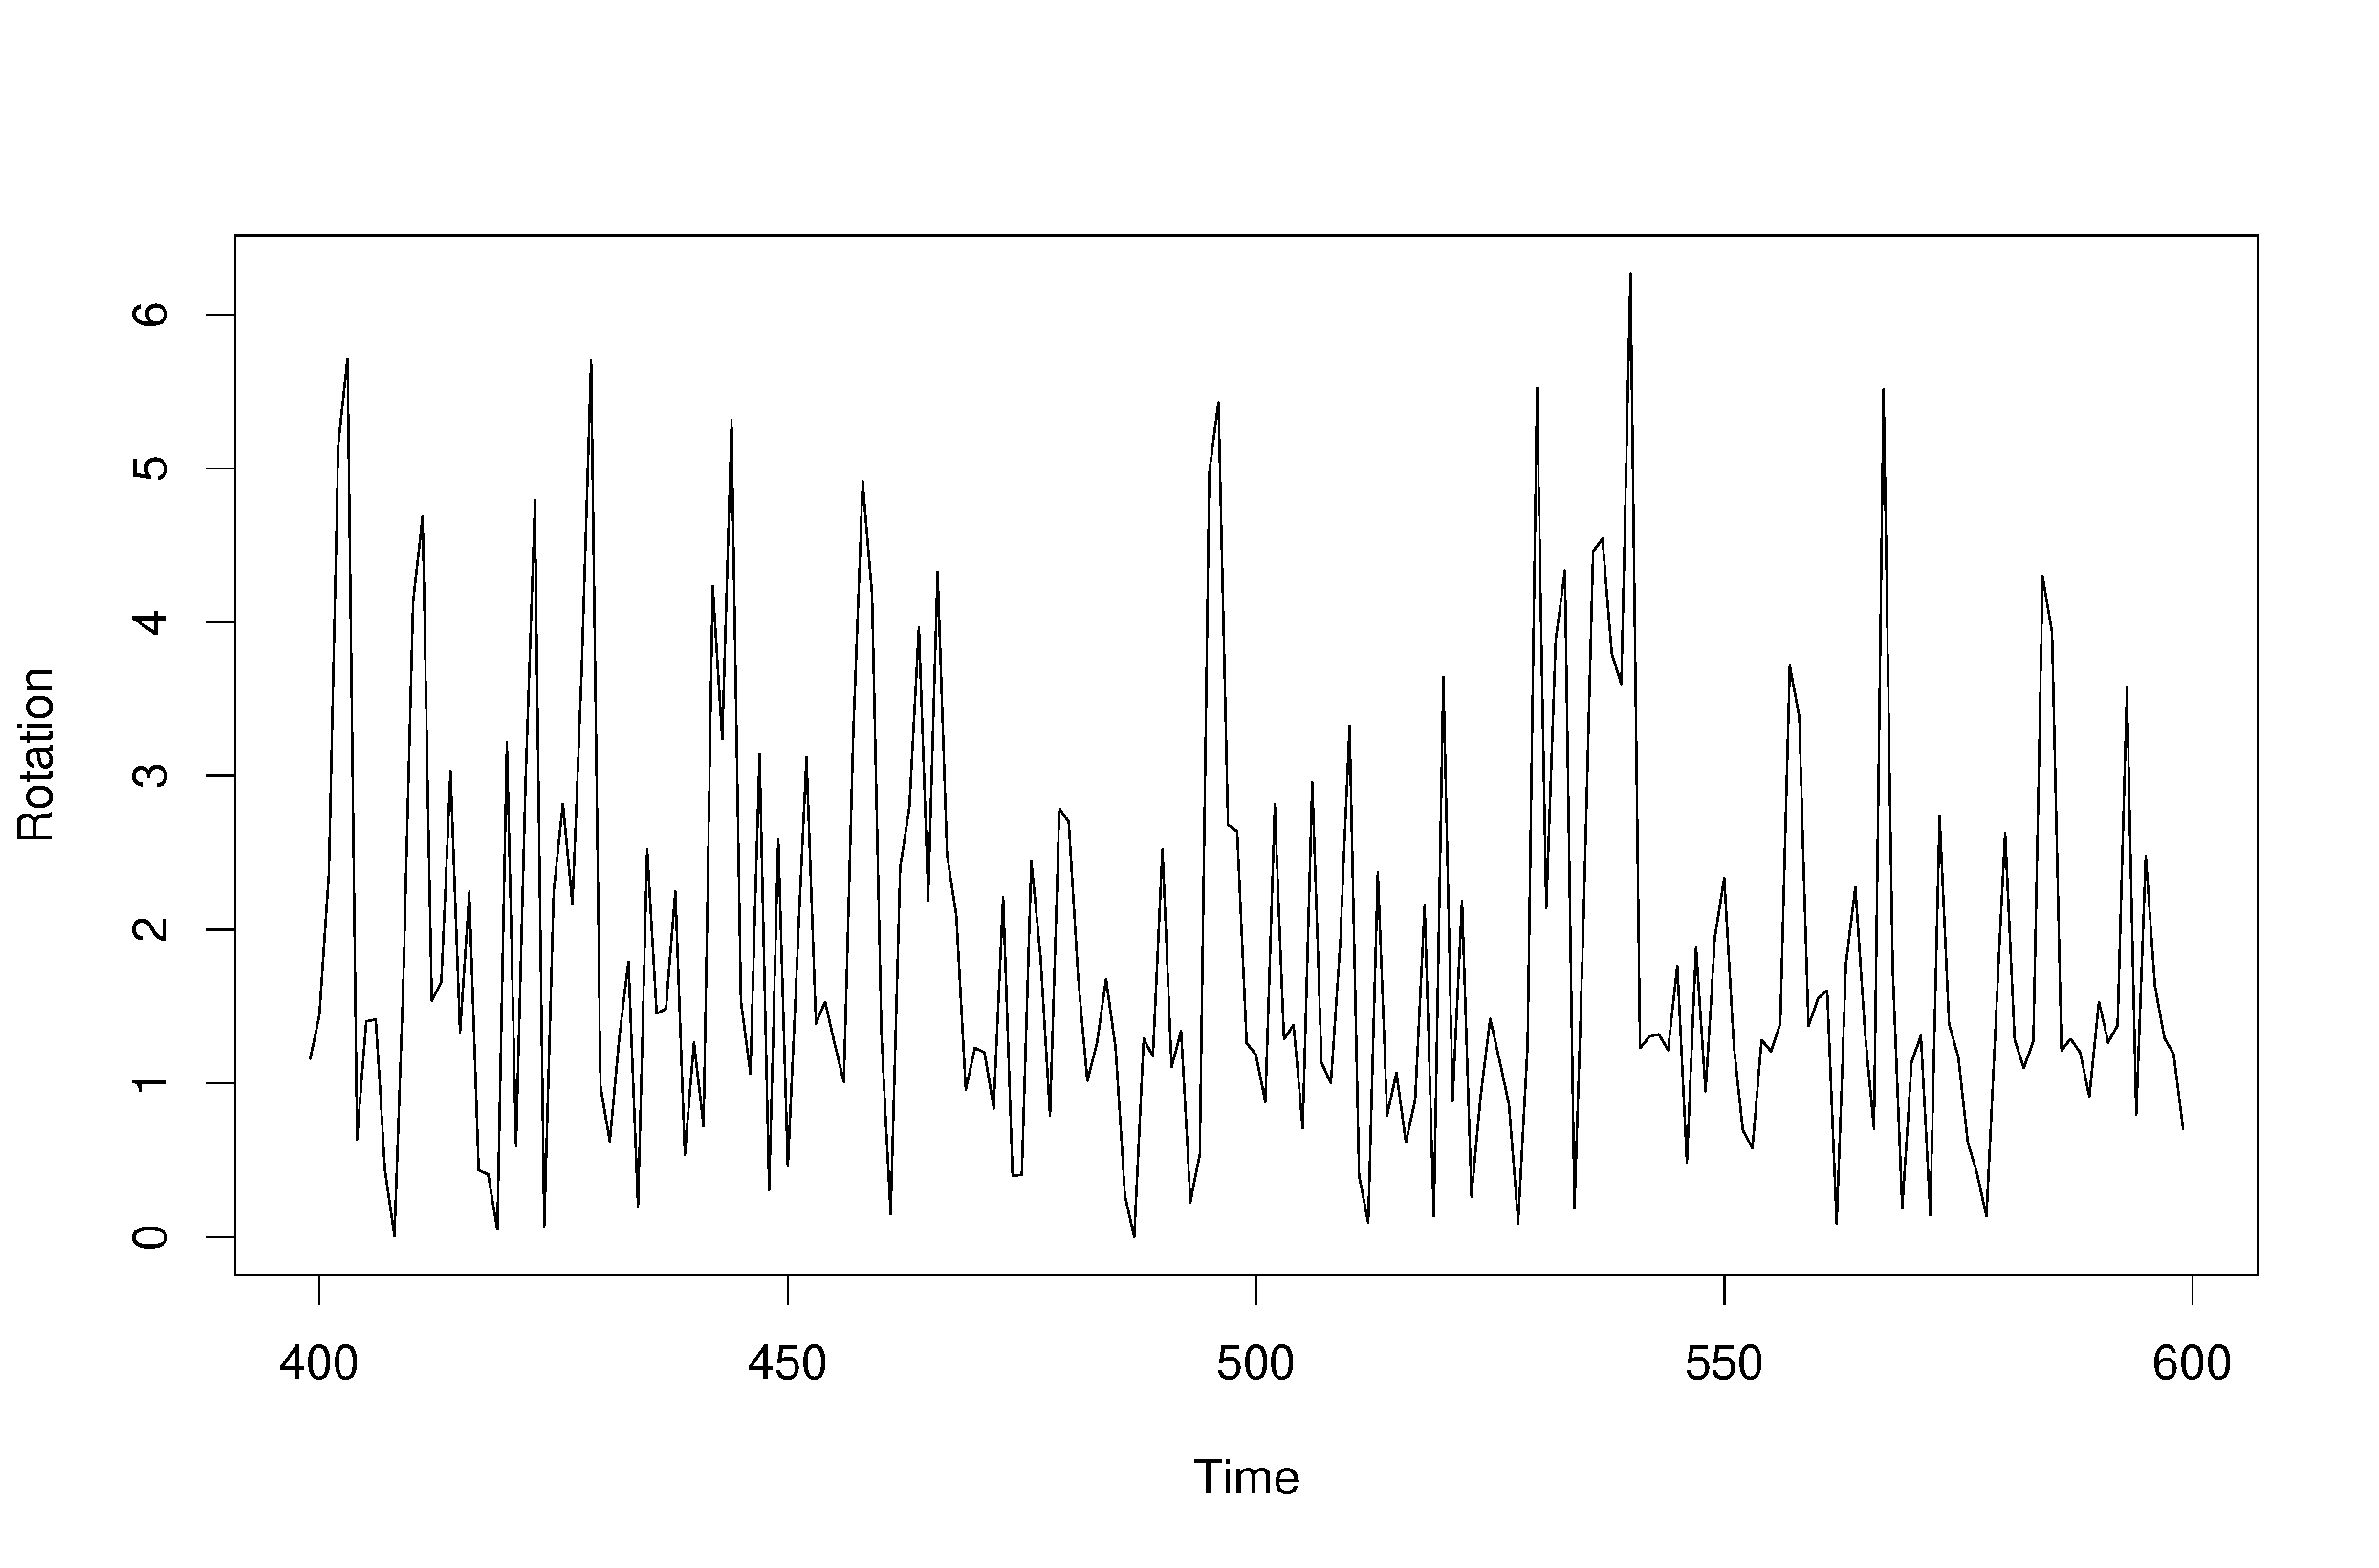
\includegraphics[width=8cm]{fig/rotation_400-600}\NN
		  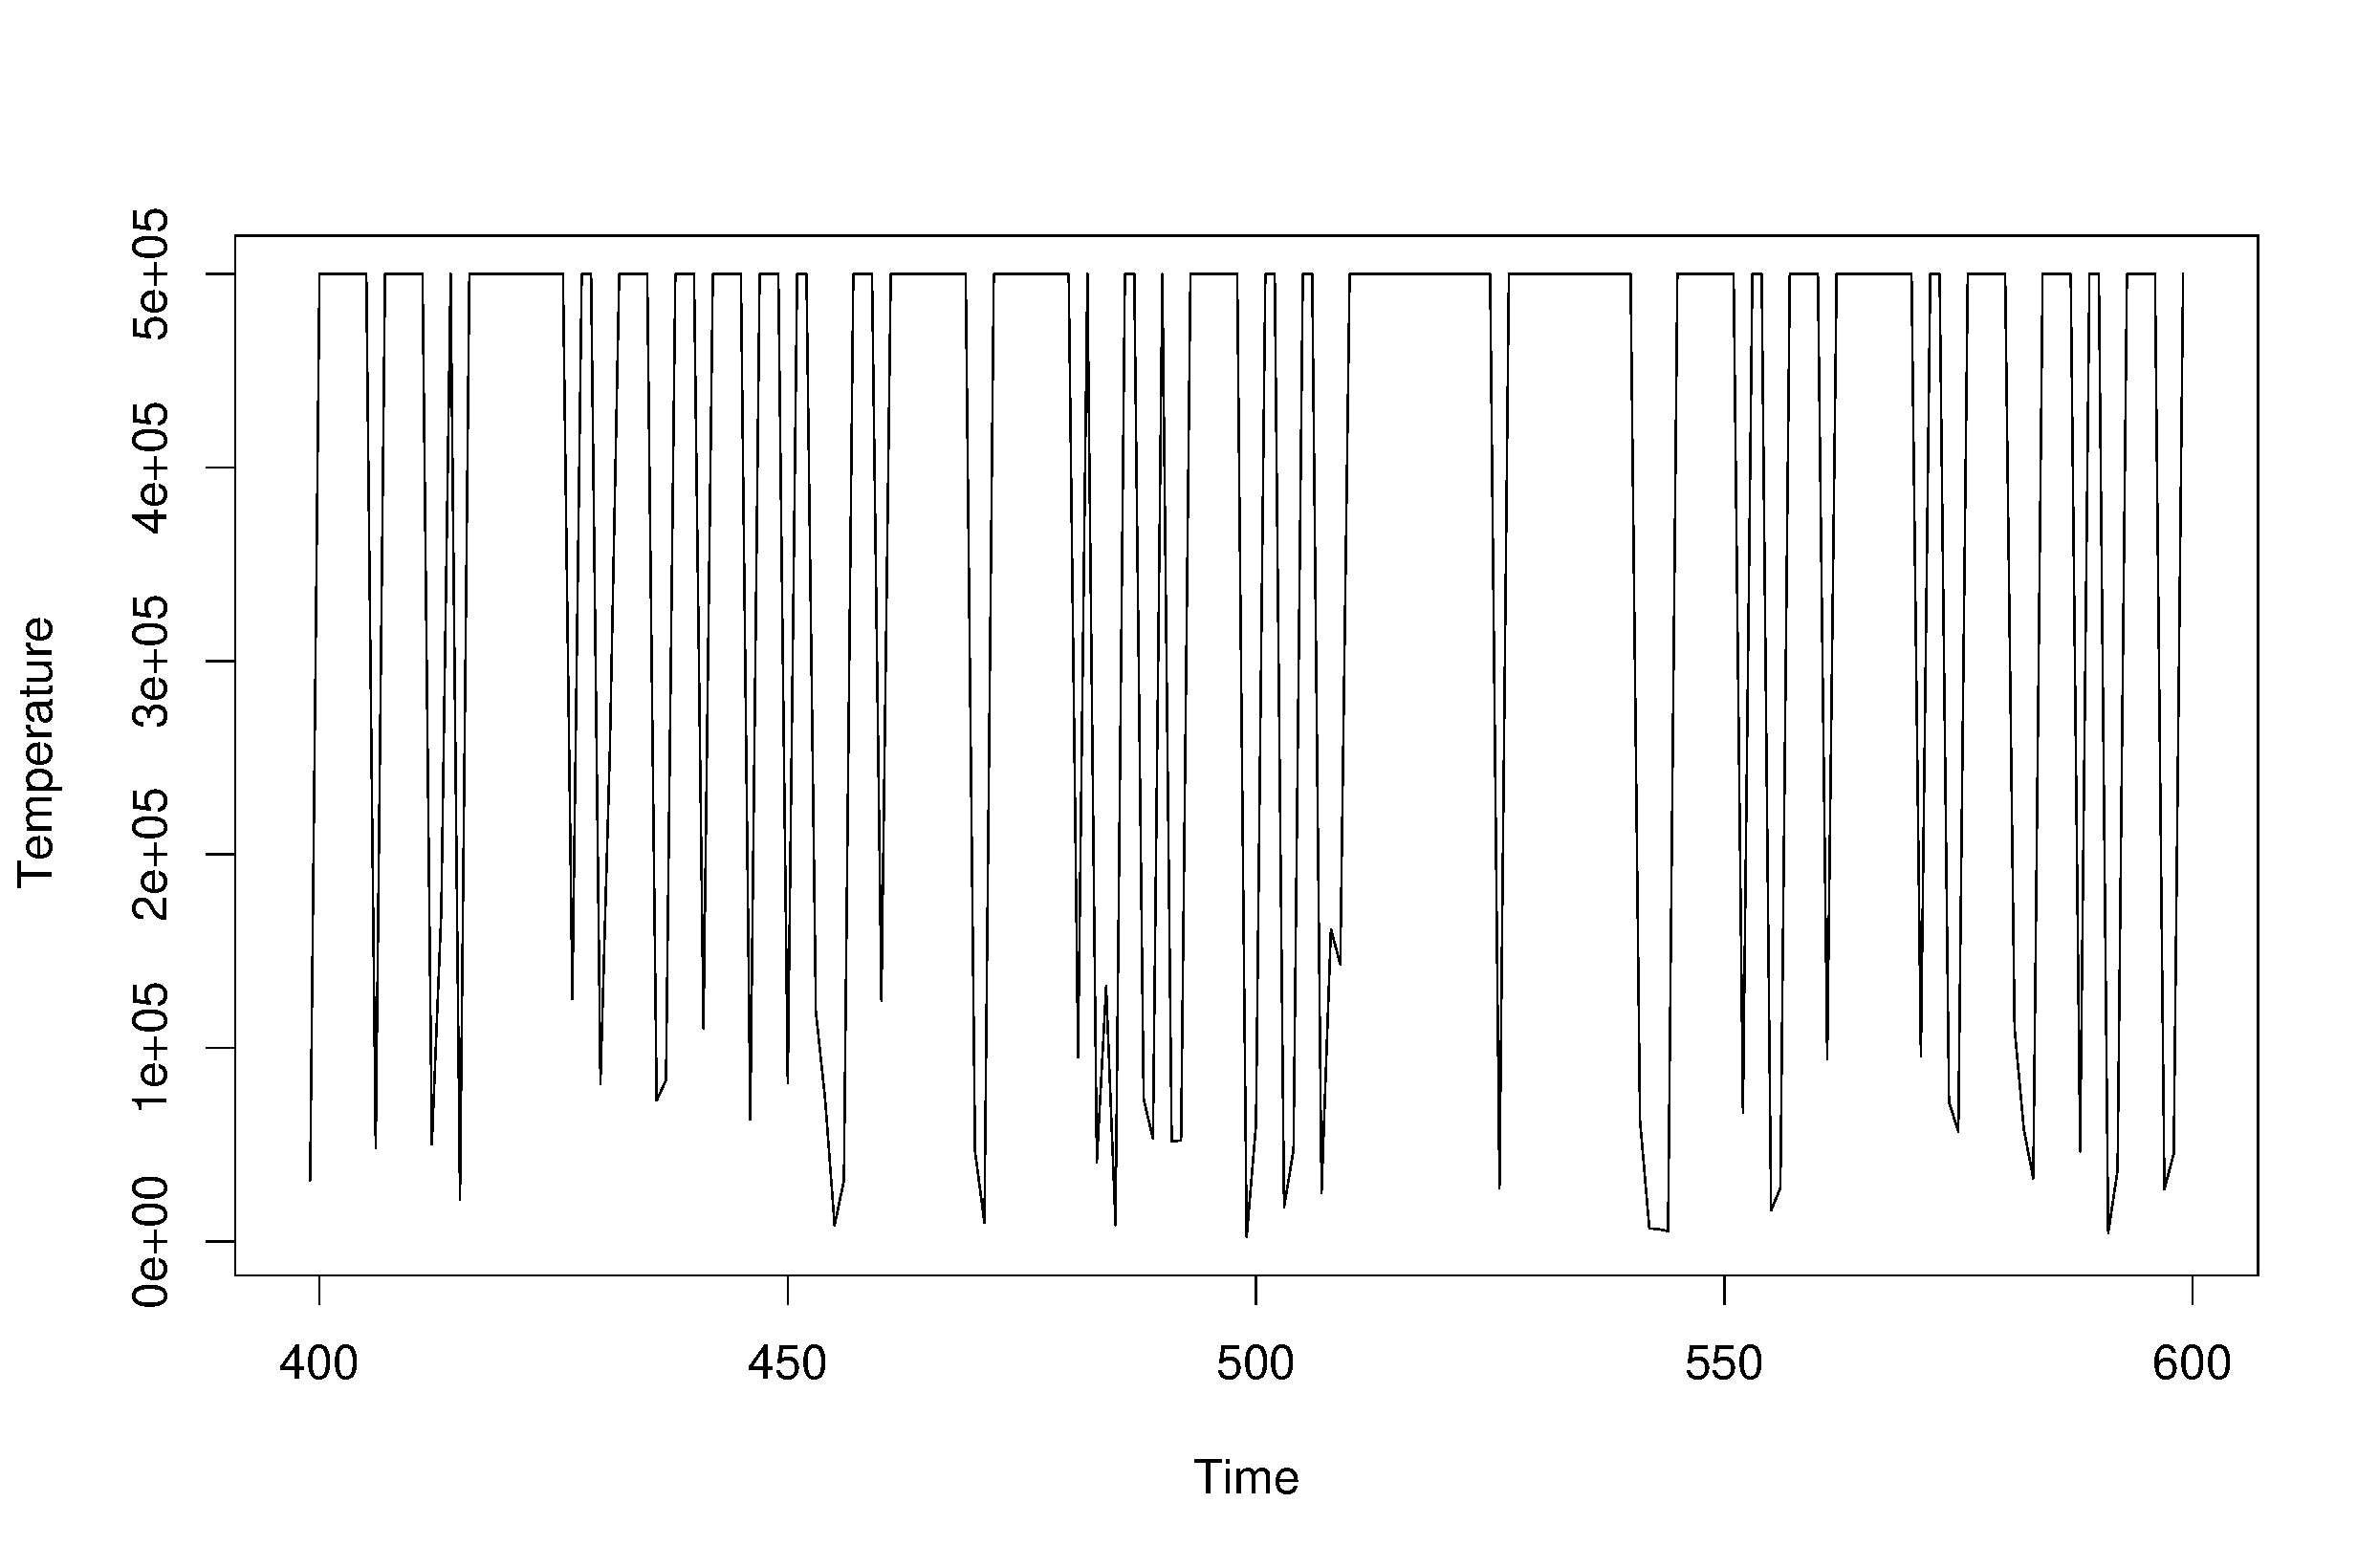
\includegraphics[width=8cm]{fig/temp_rot_400-600}\LL
		  }
\ctable[caption={The rotation angle towards the end of the TSA process},
	     figure,
		  label={fig:rot19}]{c}{\tnote[]{}}{\FL
		  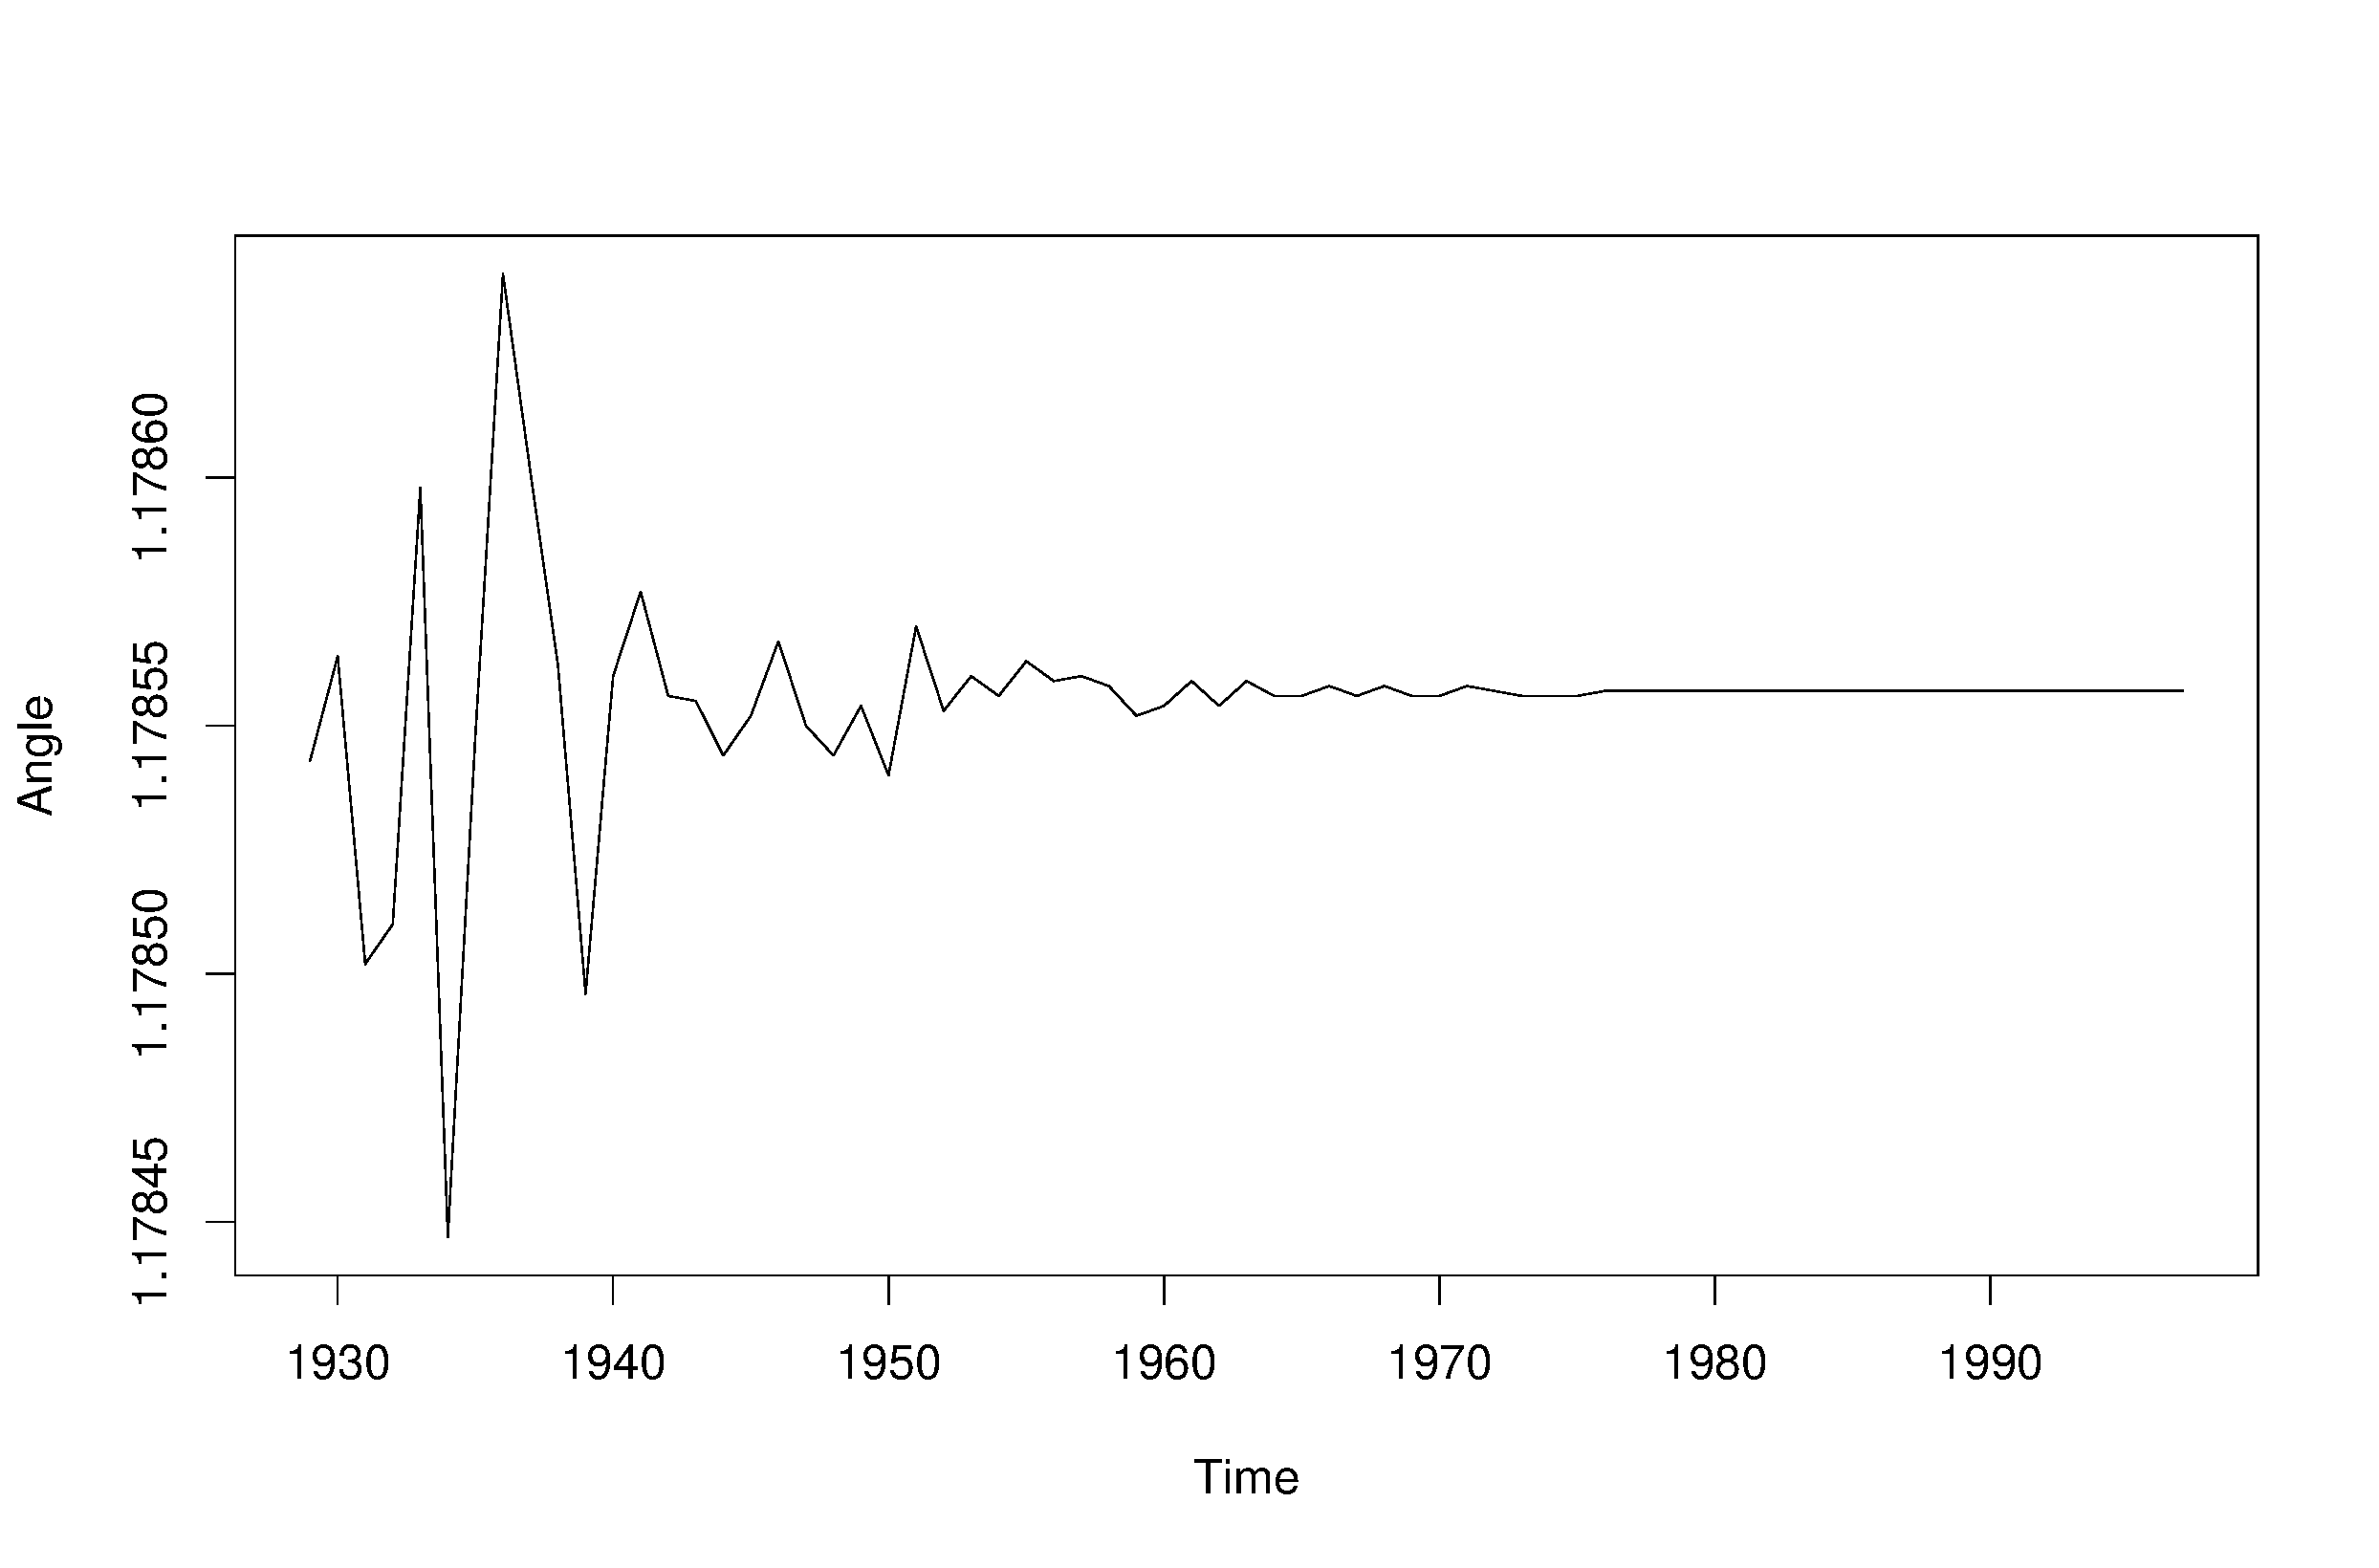
\includegraphics[width=8cm]{fig/rotation_1930-1998}\NN
		  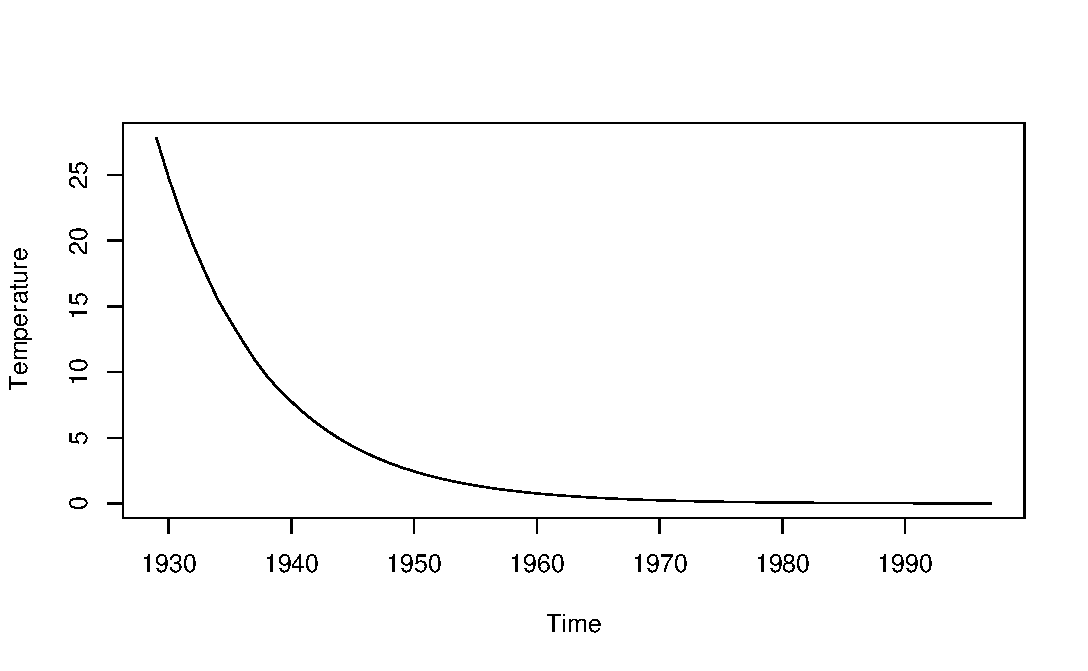
\includegraphics[width=8cm]{fig/temp_rot_1930-1998}\LL
		  }

In Fig. \ref{fig:rotful}, \ref{fig:rot46}~and \ref{fig:rot19}~the angle and
the temperature and different times is shown. The overall behaviour of the
angle over time can be seen in Fig. \ref{fig:rotful}. Equation \ref{eq:rot}~
causes the angle to behave randomly. At the beginning of the process, where
the temperature is very high, the process is very instable. This changes when
the temperature lowers. As can be seen if \ref{fig:rot46} the process seems to
`walk around' 1.2 radials. This is pure randomness. As can be seen inf Fig.
\ref{fig:rot19}~the temperature finally cools down to a minimum the movement
of the Brownian Motion also diminishes.

Perturbing the system using a Brownian Motion which influence is reduced as
the system cools, allows to jump to other angles.

\subsection{Cooling Schedule}
In the classical SA algorithm the cooling schedule has to be fine tuned to
solve each problem. However, because the renormalization algorithm is supposed
to be general purpose, we argue that fine tuning every problem is undesirable.
Therefore a auto-tuning cooling schedule is more sensible. The TSA algorithm
proposed in \cite{devicente2003pts}~implements a cooling schedule which uses
the energy variance and the entropy variance of the system to find a new
temperature. 

\subsubsection{Energy}
As previously discussed the energy of the system is defined to be the length
of the route as found by the renormalization process. While attempting to
lower the temperature the system seeks states with a lower energy. These
states are found by perturbing the current state. When a state has a lower
energy it is accepted when
\begin{equation}\label{eq:accept}
X < e^{-\Delta E / T}
\end{equation}
where $\Delta E$ is the difference between the current energy and the last
energy, $T$ is the current temperature and $X\sim N(0, 1)$. When a state is
accepted the energy change is added to the total energy variance $E_\sigma$.
Cooling the system increases the total energy variance.

\subsubsection{Entropy}
Entropy is known in field of Physics and Information Theory. In both cases it
describes the notion of inconsistency of the current state. When the system is
at a very high temperature, --in the metallurgy analogue-- the atoms are very
unstable. When the energy and the temperature reduce the atoms will become
more stable and therefore the entropy will fall. The total entropy variance
$S_\sigma$ of the system is computed as:
\begin{equation}\label{eq:entropy}
S_\sigma = S_\sigma - \frac{\Delta E}{T}
\end{equation}
Together with the energy the entropy is used to adjust the temperature of the
system.

\subsubsection{Temperature}
As long as the total energy is positive or the total entropy variance is zero
the system is reheated to the initial temperature. Once the total energy
variance drops below zero the temperature is adjusted as:
\begin{equation}\label{eq:tempadj}
T = \beta\frac{E_\sigma}{S_\sigma}
\end{equation}
with a adjustment factor $\beta$. This factor permits to control how long the
system stays in disequilibrium. 

\subsection{Conclusion}
Solving the TSP using renormalization can lead to inaccurate results. This is
caused by the distribution of the cities over the grid. To improve the
distribution of the cities over the grid the grid is rotated. The angle under
which the rotation finds place which leads to the shortest route is searched
using a probabilistic algorithm. 

By using a TSA process the optimal angle is found by first
heating the system. A stochastic process is used to keep the system in
disequilibrium while the system is warm. Once a steady state is found the
temperature is slowly cooled using an auto-adjustment algorithm.

It remains to be verified that using this method leads to shorter paths.

% vim:ft=tex:spell spelllang=en:autoindent



% vim:ft=tex:spell spelllang=en:autoindent



\section{Results}
To demonstrate the potency of our approach we have solved the TSP for multiple
datasets. We compare the optimal results to the results found using the
combination of renormalization and simulated annealing. To analyze the quality
of the proposed technique the state of the system while seeking the solution
for two different datasets is compared.

The first data set which
contains 198 cities shows an ideal run of the algorithm. The second dataset
contains 575 cities and, as we shall see, is a worst case scenario for this
algorithm.

\ctable[caption={The results found compared to the shortest route for various
	cities},
		 label={fig:results},
		 figure]{c}{}{\FL
		 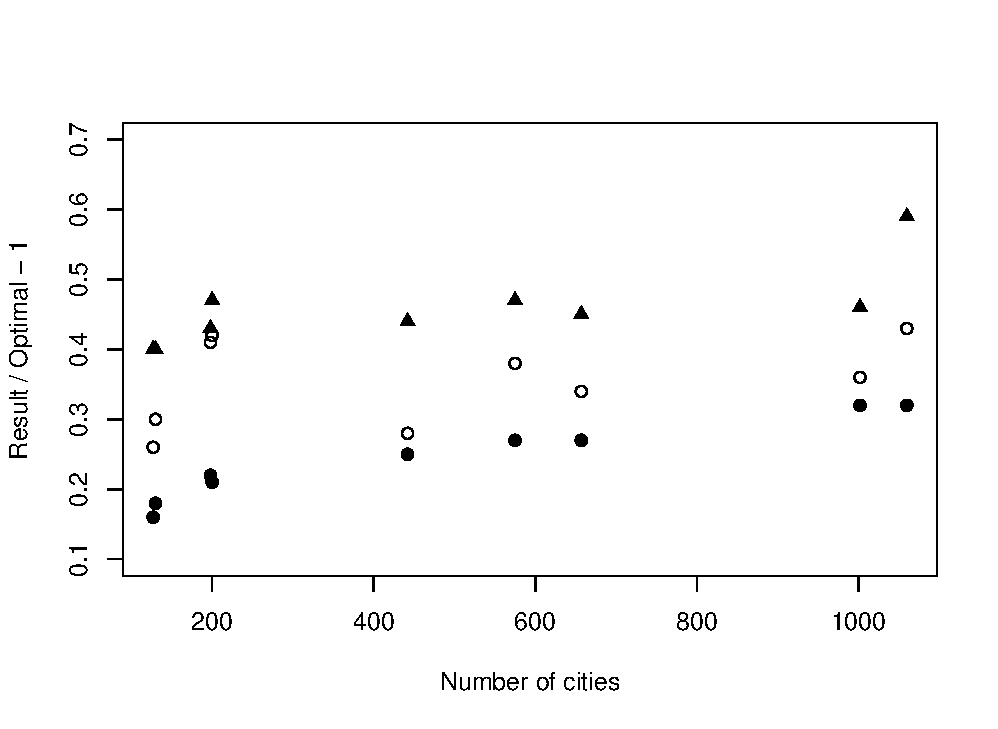
\includegraphics[width=7cm]{fig/results}
		 \LL}

\ctable[caption={The location of the cities in the 198 cities problem},
		 label={fig:d198},
		 figure]{c}{}{\FL
		 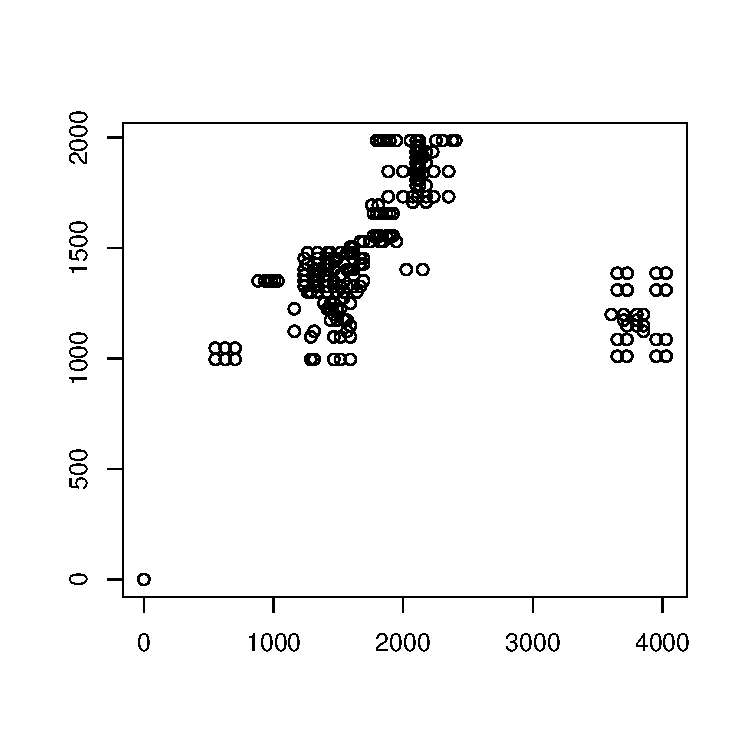
\includegraphics[width=7cm]{fig/d198cities}
		 \LL}

\ctable[caption={The location of the cities in the 575 cities problem},
		 label={fig:rat575},
		 figure]{c}{}{\FL
		 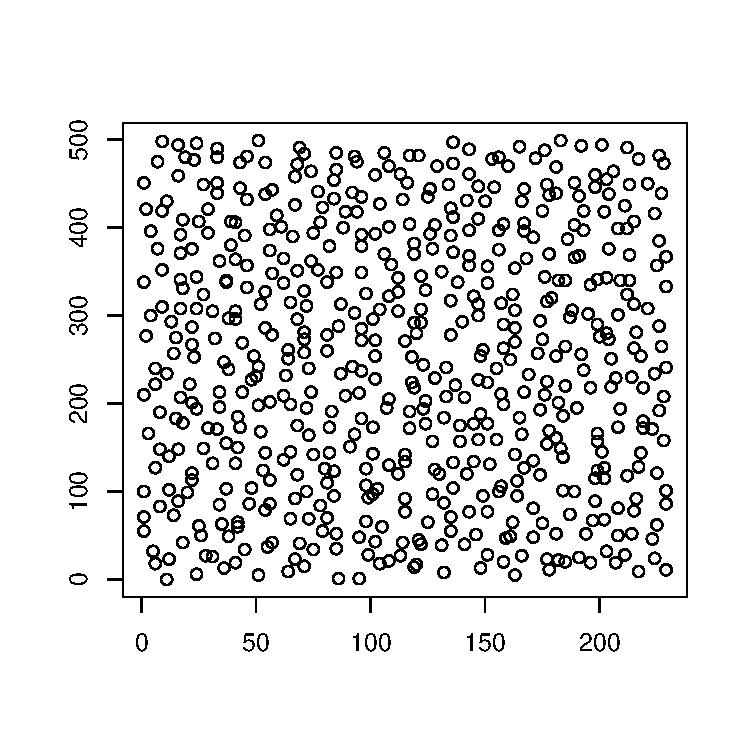
\includegraphics[width=7cm]{fig/rat575cities}
		 \LL}

\ctable[caption={Properties of the system when seeking the shortest route
		among 575 cities},
		label={fig:rat575},
		figure,
		star]{c}{}{\FL
		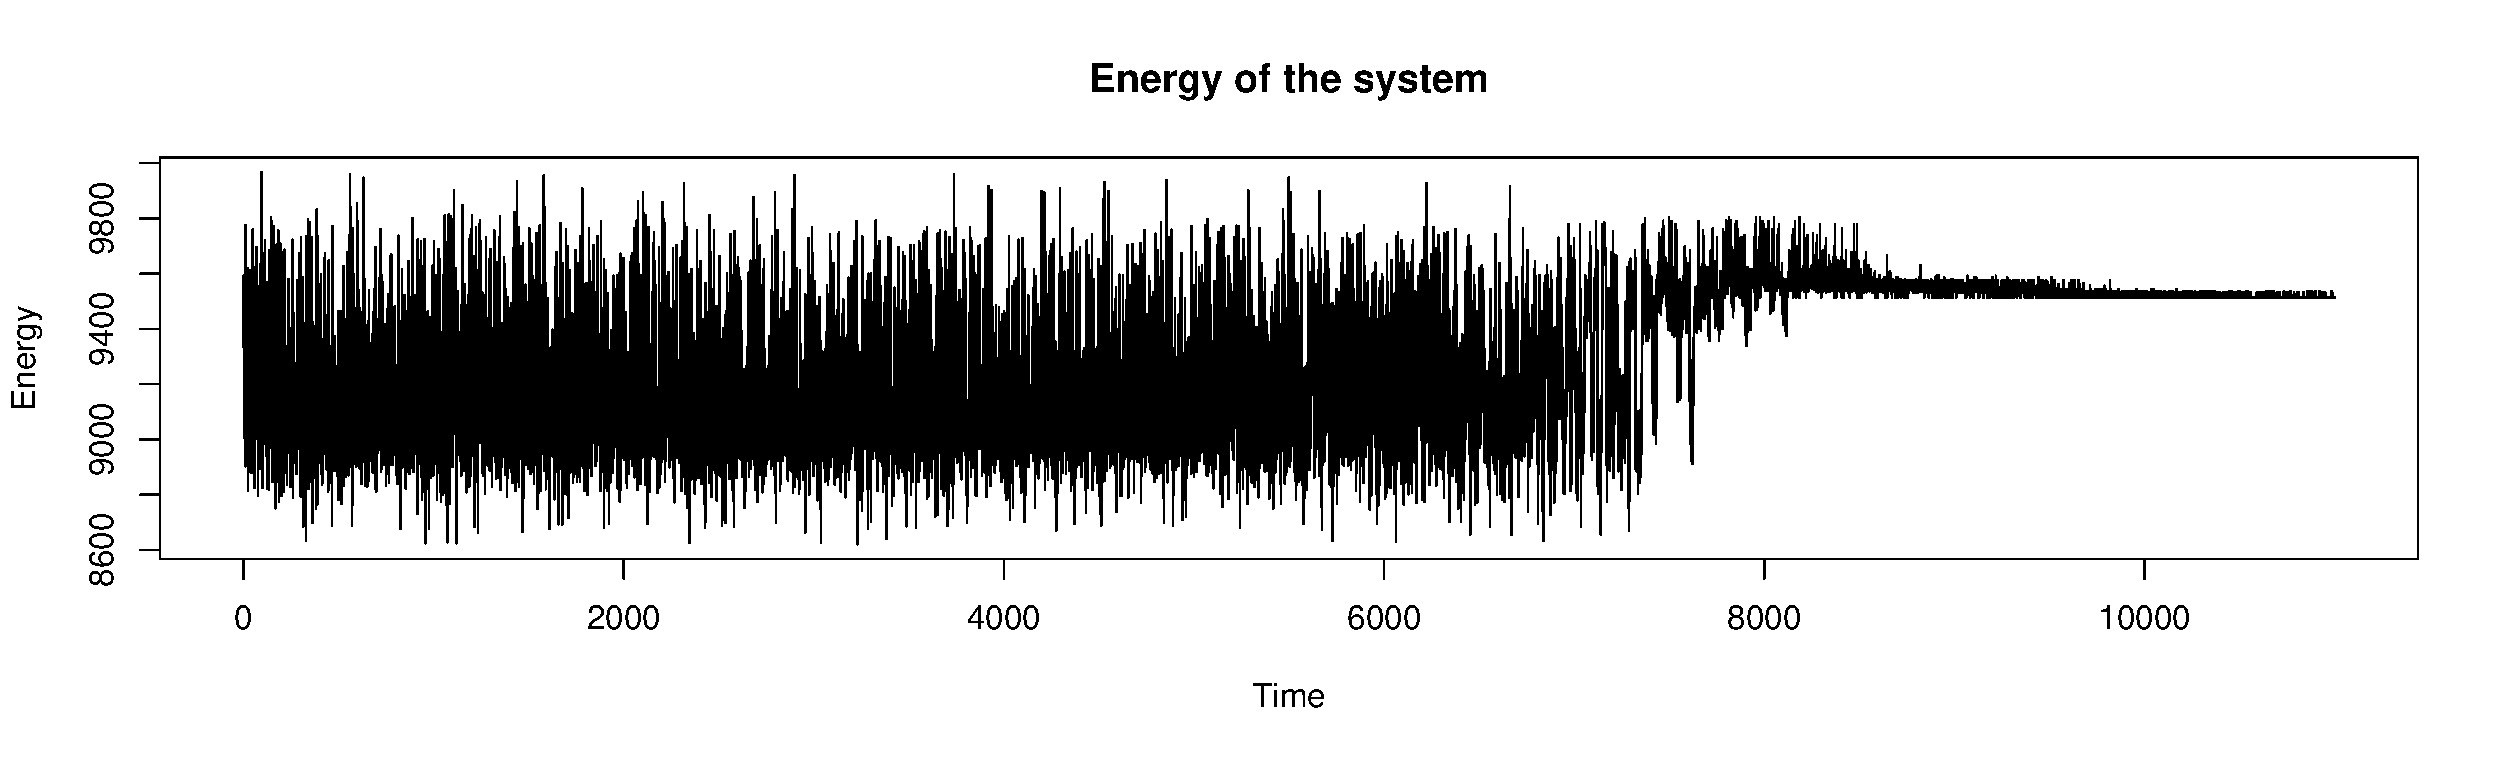
\includegraphics[width=15cm]{fig/rat575energy}\NN
		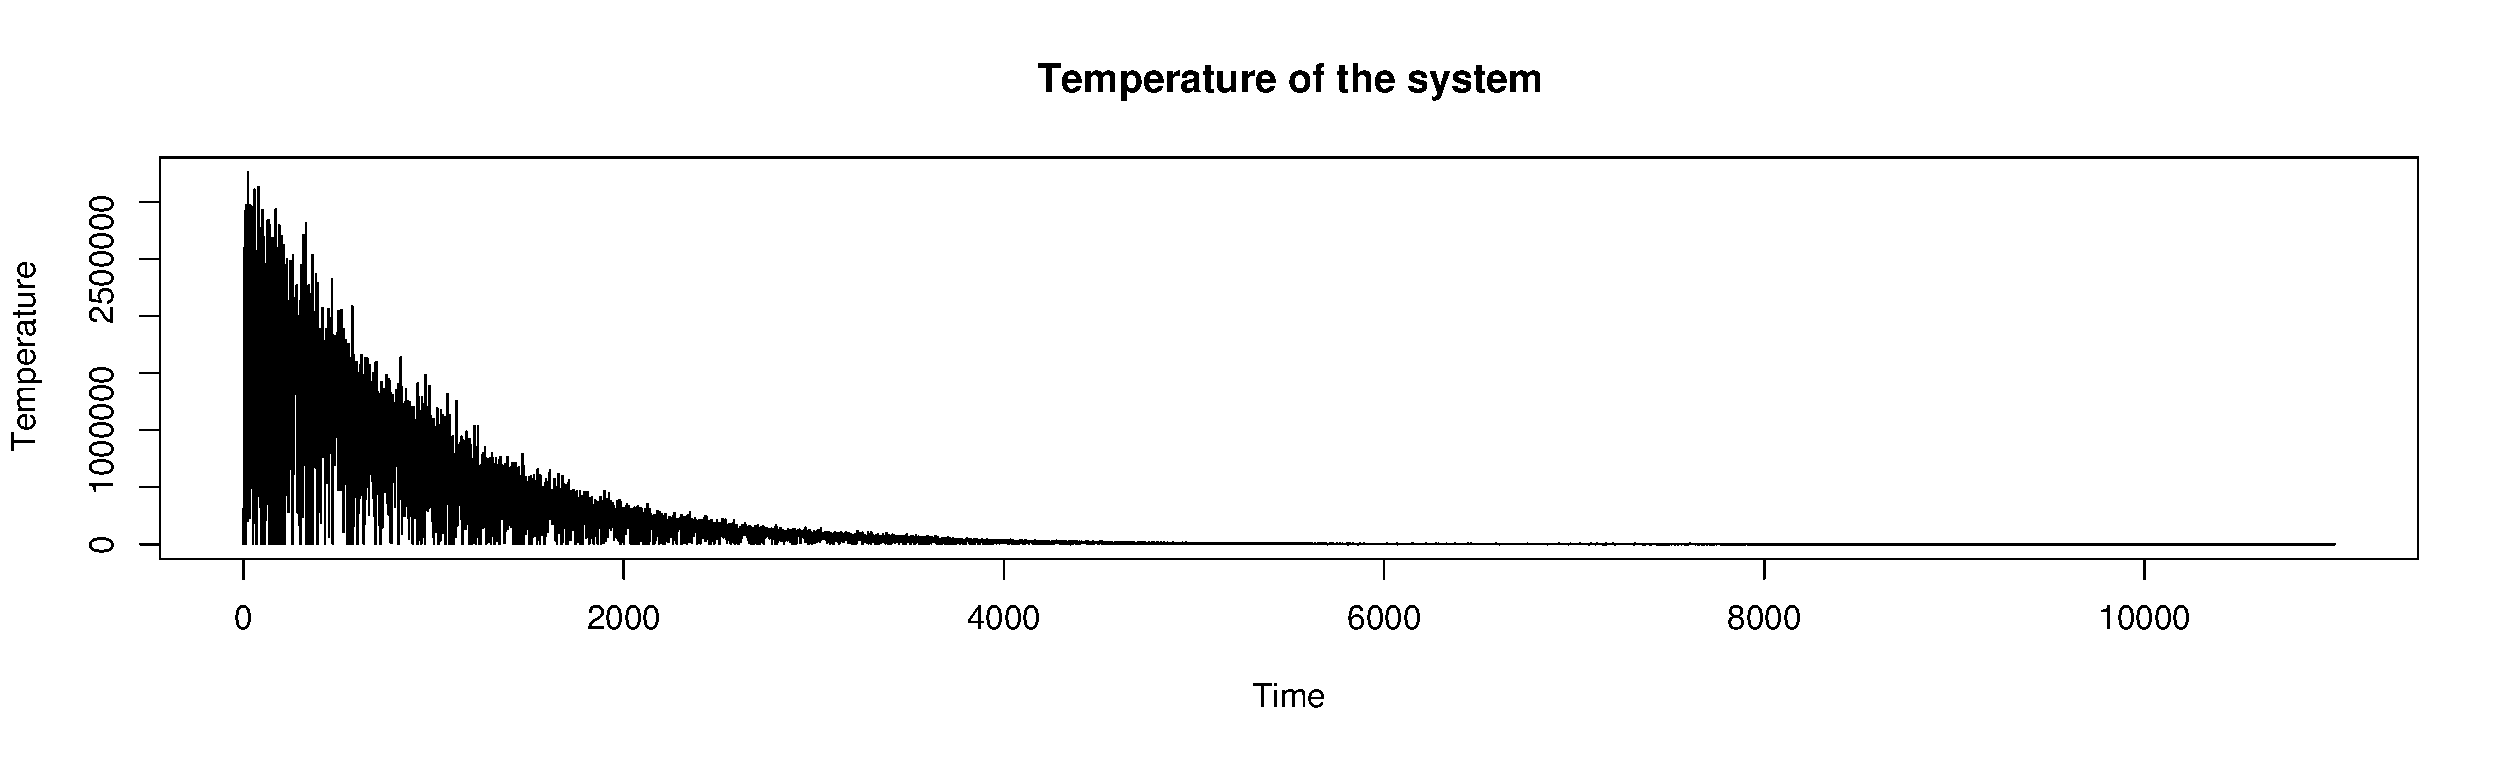
\includegraphics[width=15cm]{fig/rat575temp}\NN
		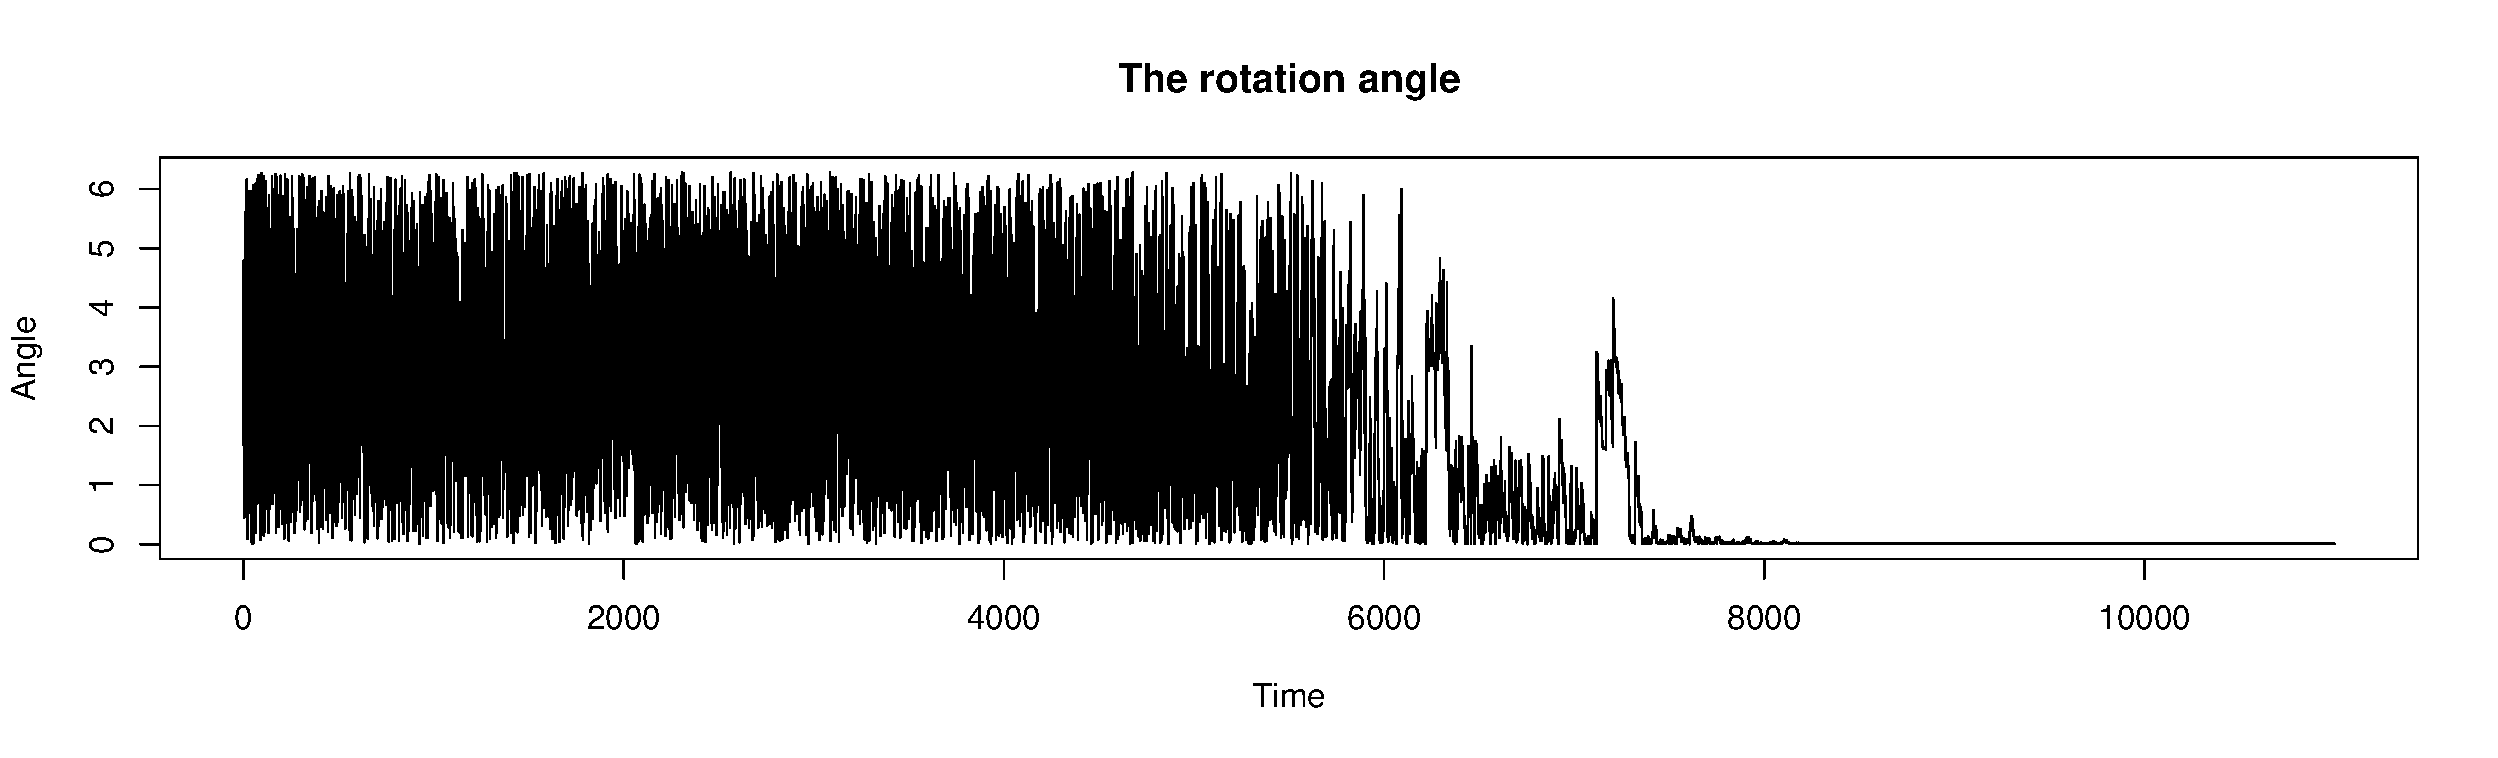
\includegraphics[width=15cm]{fig/rat575rotation}\NN
		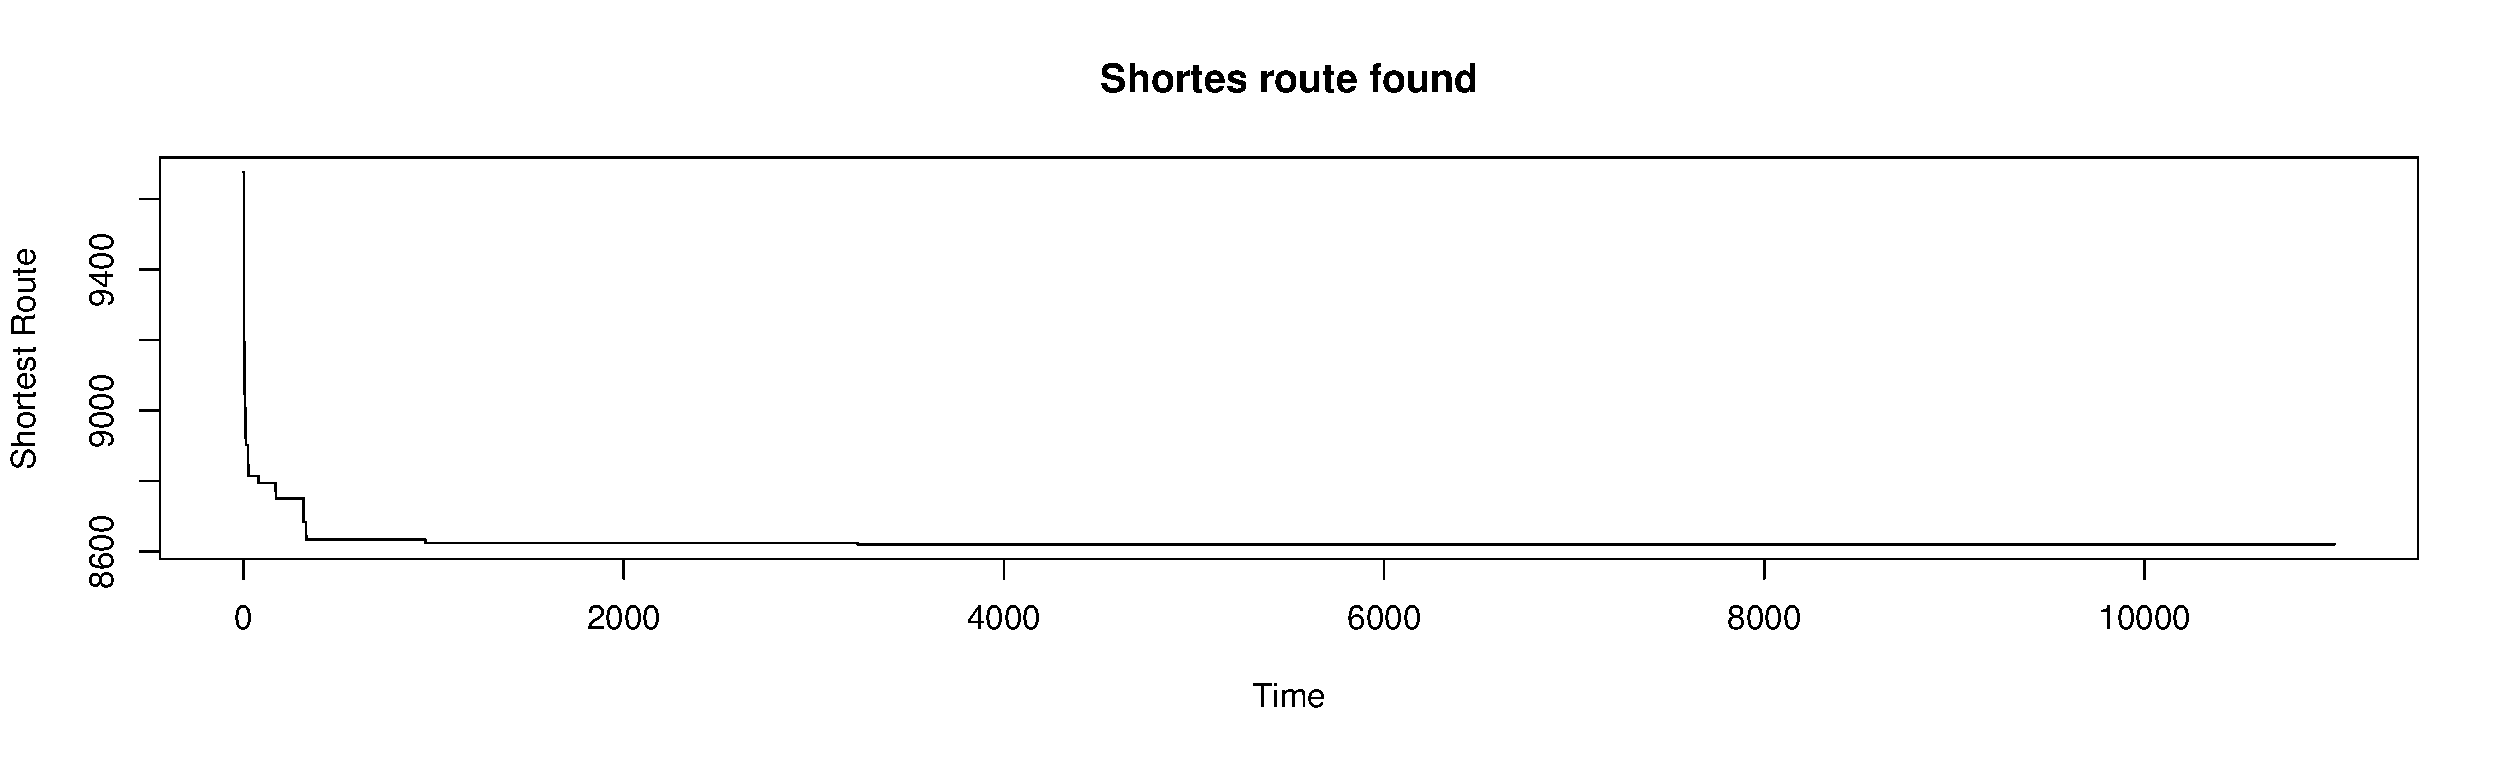
\includegraphics[width=15cm]{fig/rat575shortest}\LL}

\ctable[caption={Properties of the system when seeking the shortest route
		among 198 cities},
		label={fig:198},
		figure,
		star]{c}{}{\FL
		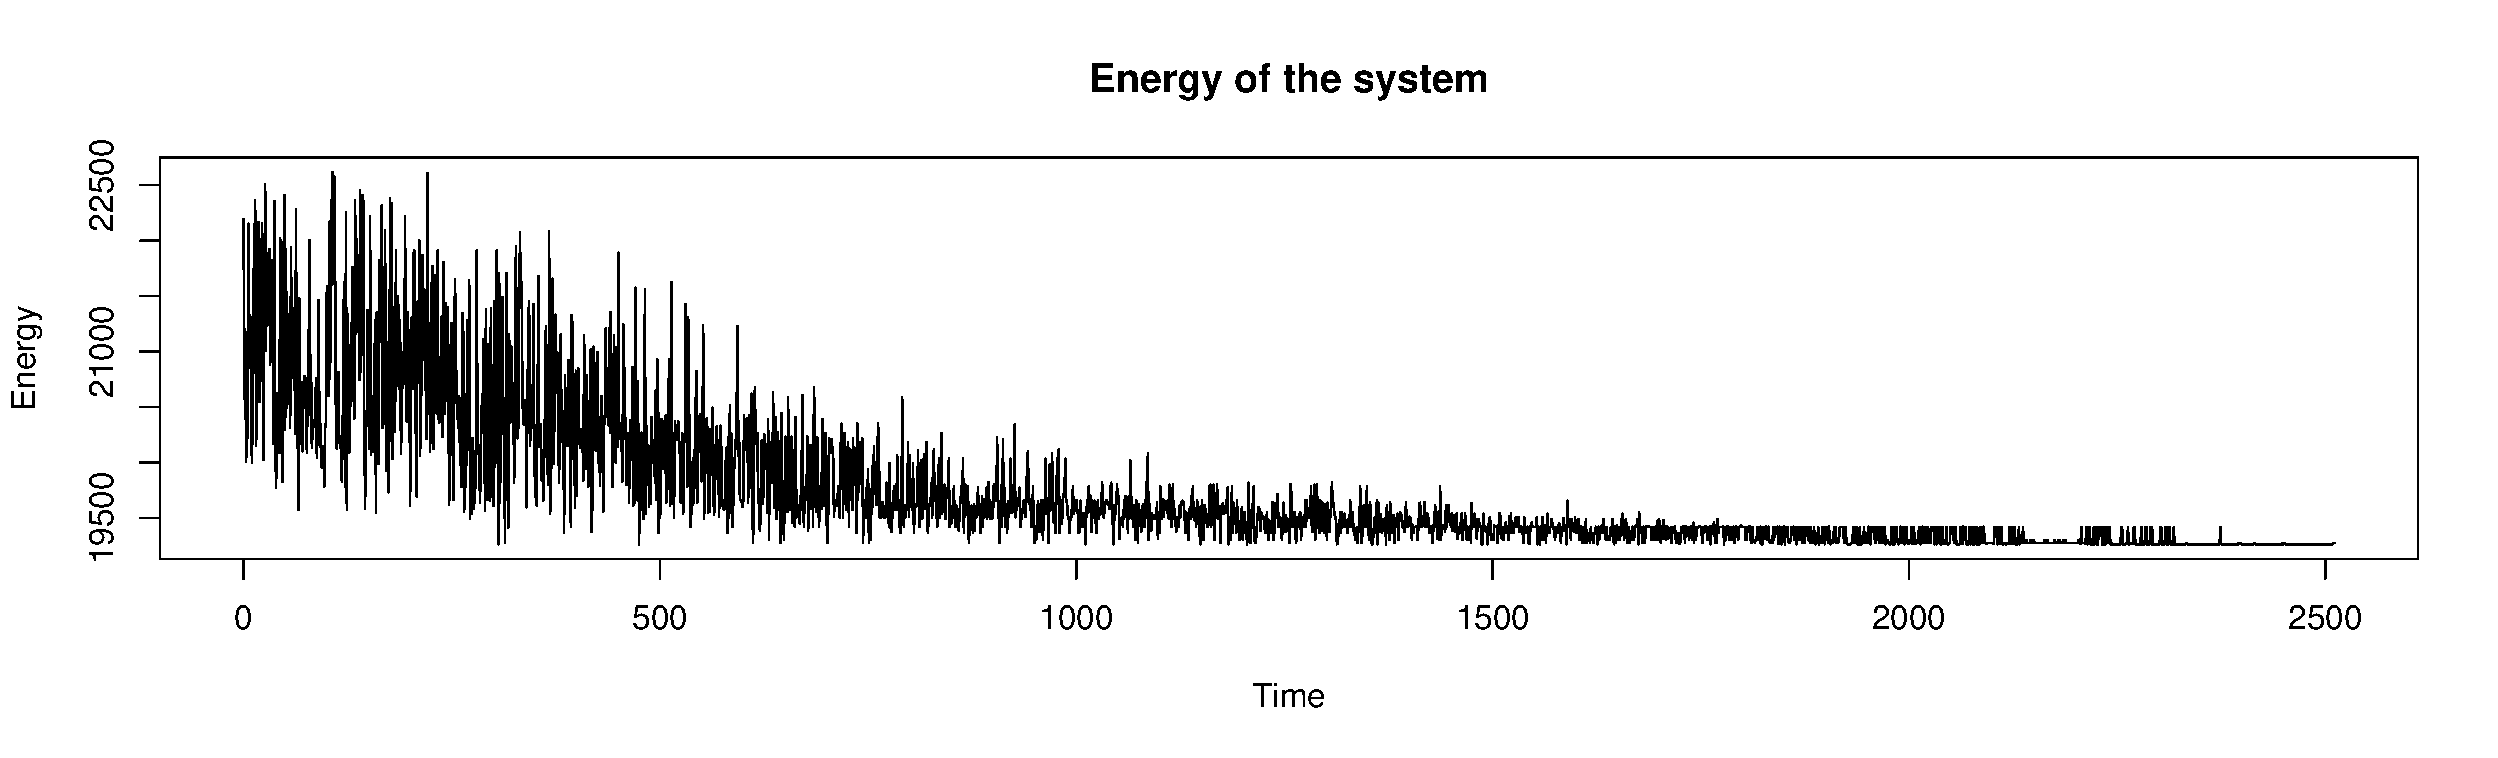
\includegraphics[width=15cm]{fig/d198energy}\NN
		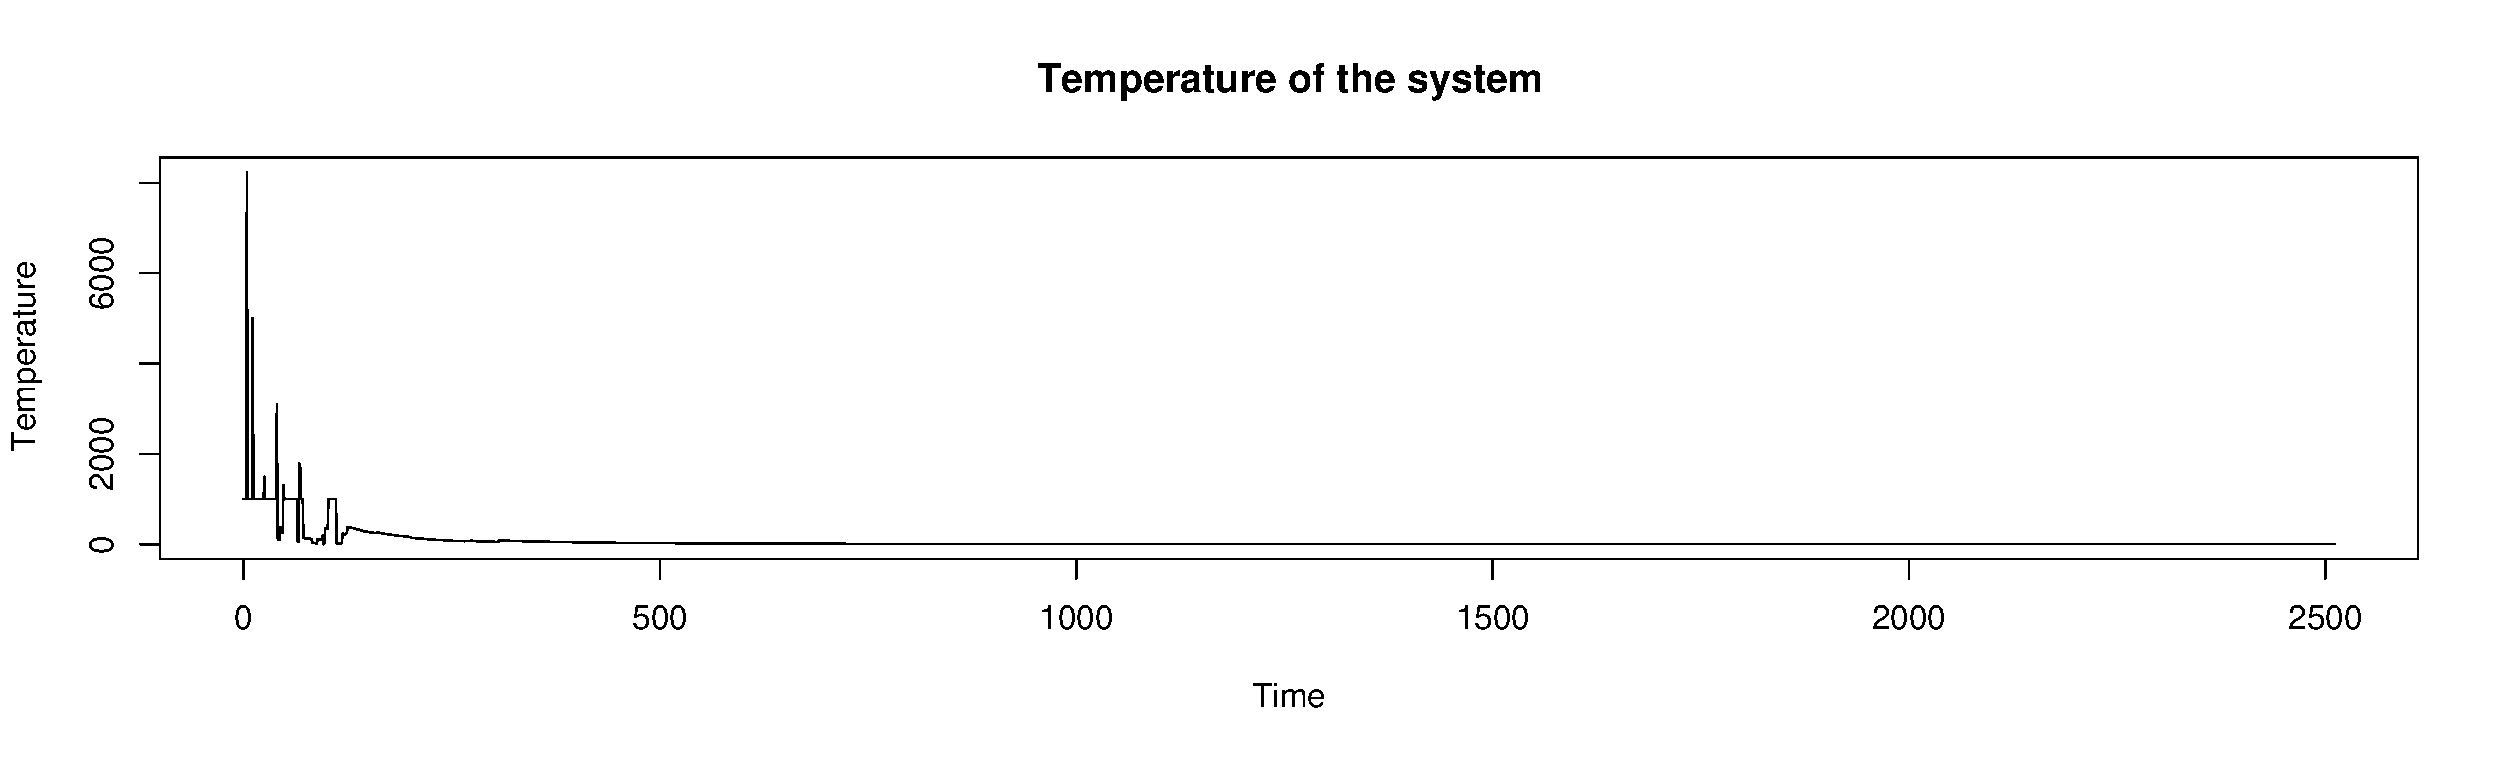
\includegraphics[width=15cm]{fig/d198temp}\NN
		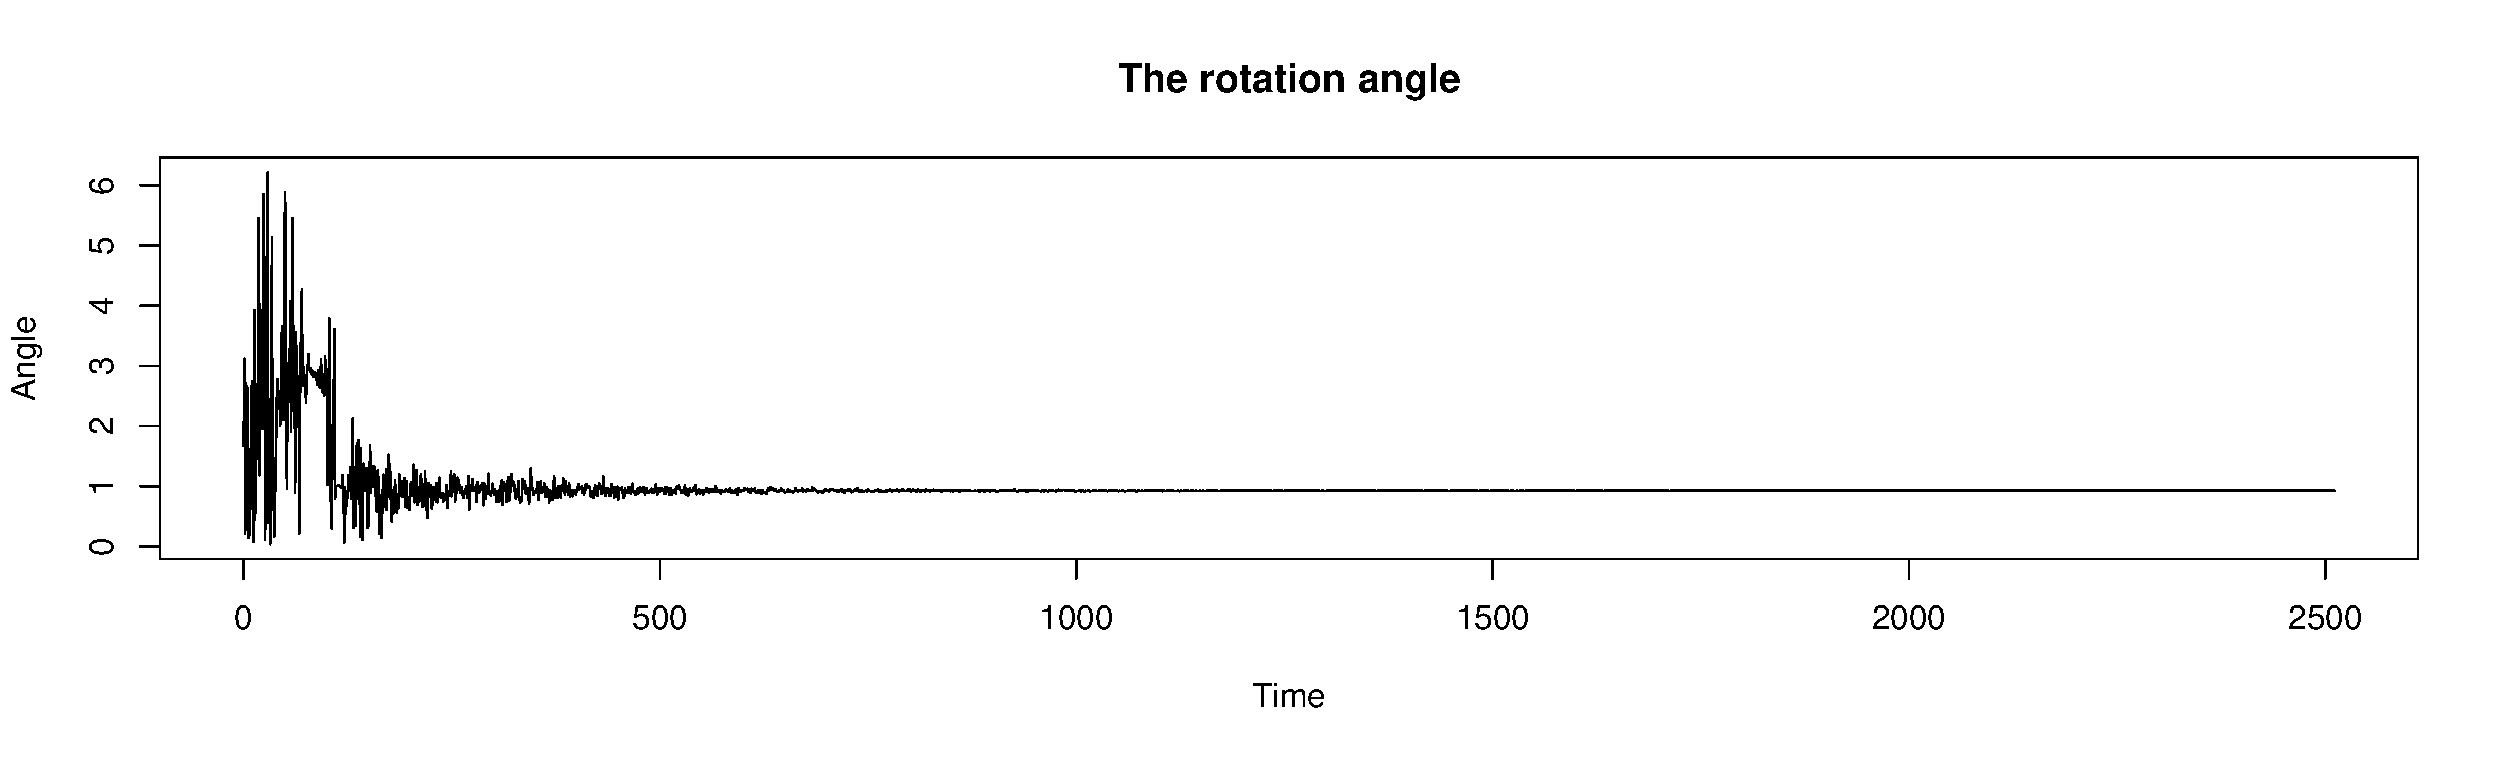
\includegraphics[width=15cm]{fig/d198rotation}\NN
		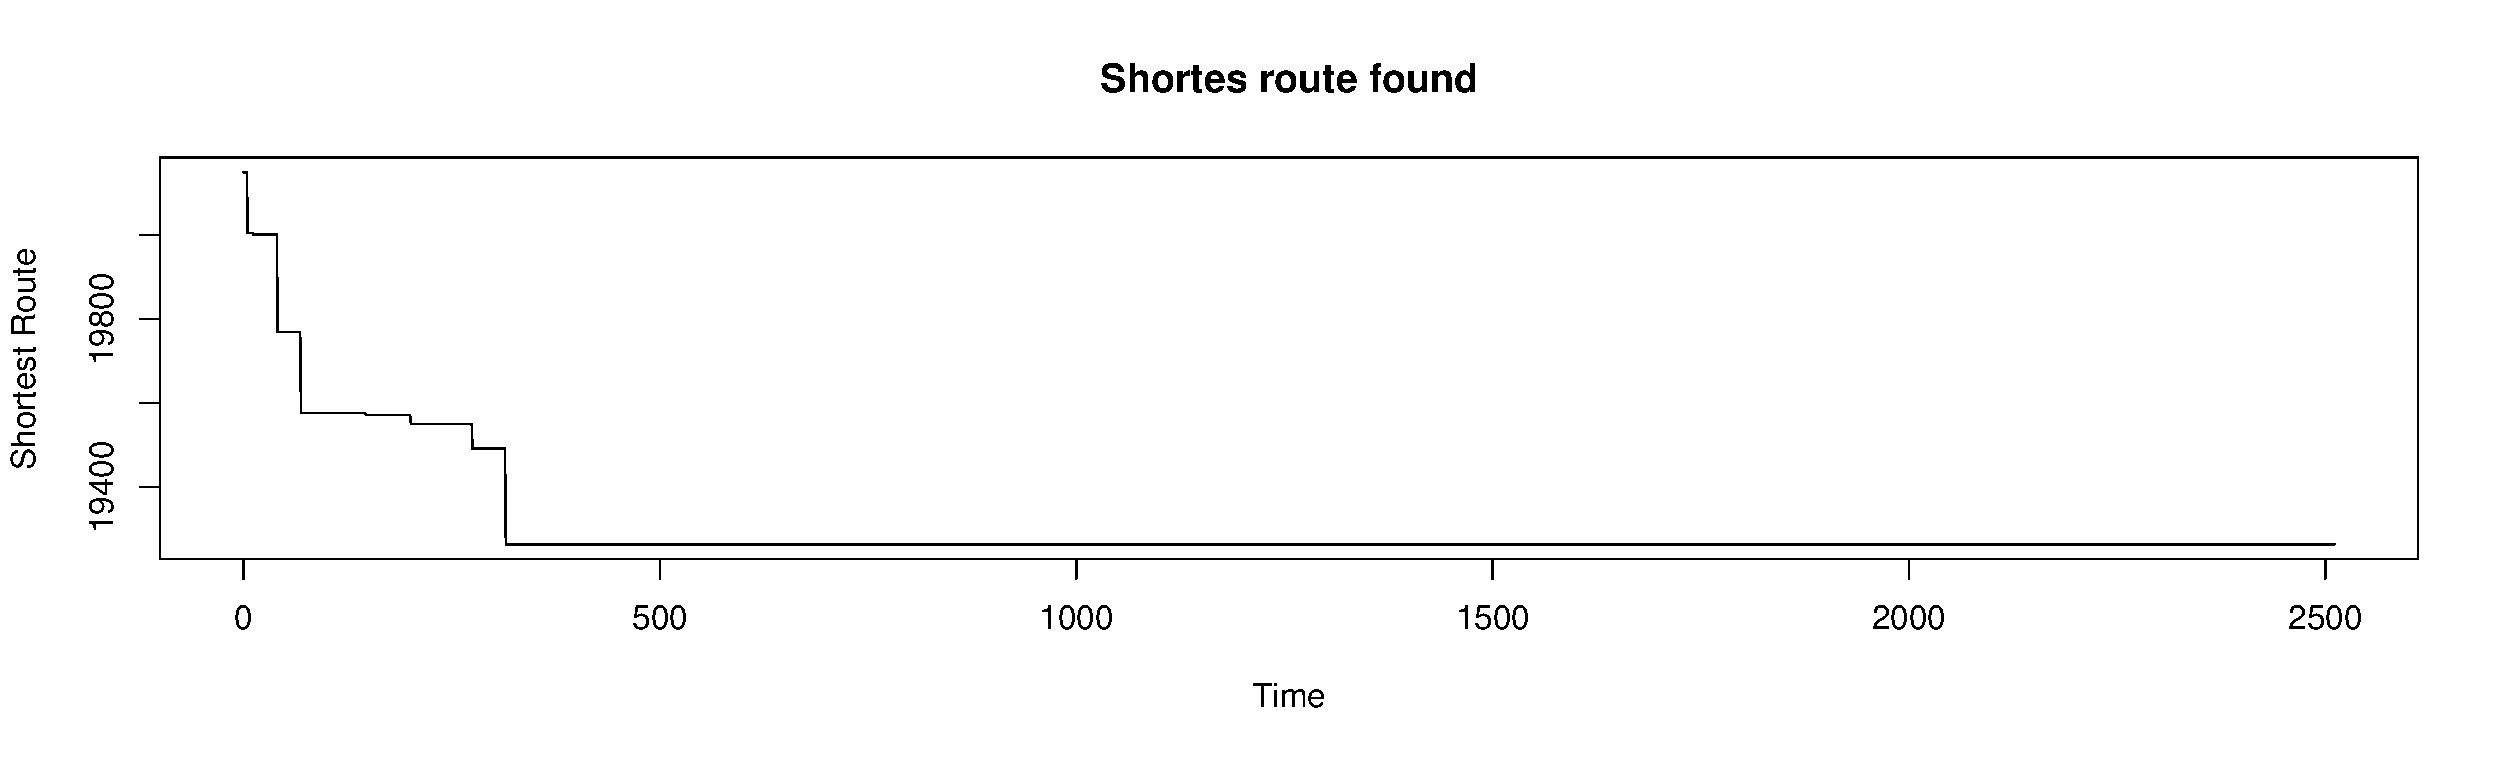
\includegraphics[width=15cm]{fig/d198shortest}\LL}


% vim:ft=tex:spell spelllang=en:autoindent



\section{Conclusion}
In this paper we have presented a method for solving the euclidean TSP. For solving the TSP we have combined Thermodynamic Simulated Annealing and Renormalization Theory. The results showed that the Renormalization Theory is a not very precise way of solving the TSP. Despite extensive search for the best rotation of the grid used in the Renormalization procedure, we got a mean accuracy of XX procent.

We can conclude that the rotation of the grid has an effect of the accuracy of the solution, but the effort of finding this correct rotation is too large. The Renormalization procedure is perfectly suited for a fast approximation of a TSP problem. This TSP problem however must fit to certain properties. TSP problems which have a large number of cities, or have clusters of cities lying close to eachother are not suited for TSP.

% vim:ft=tex:spell spelllang=en:autoindent



\bibliographystyle{IEEEtran}
\bibliography{tsp}

\end{document}

% vim:ft=tex:spell spelllang=en:autoindent

